\documentclass[12pt]{article}

% --- Encoding / fonts (fixes OT1 issues + improves monospace metrics) ---
\usepackage[T1]{fontenc}
\usepackage{lmodern}

% --- Math ---
\usepackage{amsmath}
\usepackage{amssymb}
\usepackage{graphicx}

% --- Tables ---
\usepackage{tabularx}

% --- Diagrams ---
\usepackage{tikz}
\usetikzlibrary{arrows.meta, positioning, fit, backgrounds, calc, shapes.geometric, patterns, decorations.pathreplacing}

% --- Layout ---
\usepackage{geometry}
\geometry{a4paper, margin=1in}

% --- Better line breaking / fewer overfull boxes ---
\usepackage{microtype}
\emergencystretch=2em % last-resort "be less picky" knob for line breaks

% --- Links and cross-refs ---
\usepackage[colorlinks=true,linkcolor=blue,urlcolor=blue,citecolor=blue]{hyperref}
\usepackage[nameinlink,noabbrev]{cleveref}

% --- Convenience for inline code that may need breaks ---
\newcommand{\code}[1]{\texttt{#1}}

% --- Code listings ---
\usepackage{listings}
\lstset{
  language=C++,
  basicstyle=\small\ttfamily,
  keywordstyle=\bfseries,
  commentstyle=\itshape,
  columns=flexible,
  keepspaces=true,
  breaklines=true,
  frame=none,
  aboveskip=0.5\medskipamount,
  belowskip=0.5\medskipamount,
  morekeywords={__global__,__device__,__host__,__fmaf_rd,__fmaf_rn,
                blockIdx,blockDim,threadIdx,uint32_t,size_t}
}

\newcommand{\FractalShark}{\textit{FractalShark}}

\title{\FractalShark{}: High-Performance Mandelbrot Rendering}
\author{Matthew Renzelmann}
\date{\today}

\begin{document}

\maketitle

\vspace{1em}

\begin{center}
\textit{These notes are a work-in-progress summary of \FractalShark{}. Moreover,
much of it is presently AI-generated and thus may contain errors or
inconsistencies.  That said, I've made some effort to review and correct it, so
it should be better than nothing.  I'll remove this warning once I'm better
satisfied with the content.  This document has seen significant revisions
recently and is getting better.}
\end{center}

\renewcommand\numberline[1]{#1\enspace}

\tableofcontents
\listoffigures
\listoftables
\clearpage

\section{Notation}
\label{sec:notation}

The following symbols appear throughout these notes.  Where a concept
admits more than one notation the table lists the canonical form first
and notes the section-local variant.

\begin{table}[!htbp]
\centering
\caption[General notation]{General notation used throughout these notes.}
\label{tab:notation-general}
\small
\begin{tabularx}{\textwidth}
    {l>{\raggedright\arraybackslash}p{0.34\textwidth}>{\raggedright\arraybackslash}X}
\hline
\textbf{Symbol} & \textbf{Meaning} & \textbf{Notes} \\
\hline
$z_n$        & orbit value at iteration $n$  & $z_0=0$,\; $z_{n+1}=z_n^2+c$ \\
$c$          & complex parameter (pixel)     & \\
$z_n^\star,\; c_\star$ & reference orbit / parameter
             & $z^{(0)}_n,\; c_0$ in the reuse hierarchy (\cref{subsec:ref-orbit-reuse}) \\
$\Delta z_n$ & perturbation $z_n - z_n^\star$ & \\
$\delta z_n$ & second-level perturbation      & relative to an intermediate orbit (\cref{subsec:ref-orbit-reuse}) \\
$\Delta c$   & parameter offset $c - c_\star$ & \\
$d_n \equiv \partial z_n/\partial c$ & orbit derivative
             & $d_0=0$;\; implementation starts from $d_1=1$ \\
$c^*$        & nucleus of a hyperbolic component & distinct from $c_\star$ \\
$n$          & iteration index               & \\
$p$          & period                        & \\
$n_{\text{smooth}}$ & smooth (fractional) iteration count
             & $n_{\text{smooth}} = n - \log_2\!\log_2|z_n| + \mathrm{const}$;\;
               continuous coloring \\
$N$          & generic multi-precision limb count  & section-local unless a type fixes the limb width \\
$D$          & effective number of 32-bit \code{HpSharkFloat} limbs
             & selected at runtime within a compile-time
               \code{GlobalNum\allowbreak Uint32} storage bucket \\
$L$          & number of packed base-$2^b$ coefficients
             & $L=\lceil 32D/b\rceil$ \\
$M$          & active power-of-two NTT length in the fused schedule
             & contains the complete shifted convolution support; an unshifted product needs
               $M\ge 2L-1$, rounded to a power of two, up to $2^{25}$ \\
$b$          & packed NTT coefficient width in bits
             & $b=16$ for the CUDA reference engine and its host reference model \\
\hline
\end{tabularx}
\end{table}

\begin{table}[!htbp]
\centering
\caption[Real and imaginary component notation]{Real and imaginary component notation.}
\label{tab:notation-components}
\begin{tabularx}{\textwidth}{llX}
\hline
\textbf{Symbol} & \textbf{Meaning} & \textbf{Notes} \\
\hline
$x_n,\; y_n$     & components of $z_n = x_n + i\,y_n$
                  & similarly $x_n^\star, y_n^\star$ for $z_n^\star$ \\
$\Delta x_n,\; \Delta y_n$ & components of $\Delta z_n$
                  & $\Delta c_x, \Delta c_y$ for $\Delta c$ \\
$d_{x,n},\; d_{y,n}$ & components of $d_n$
                  & \\
\hline
\end{tabularx}
\end{table}

\begin{table}[!htbp]
\centering
\caption[Linear approximation notation]{Linear approximation notation.}
\label{tab:notation-la}
\begin{tabularx}{\textwidth}{llX}
\hline
\textbf{Symbol} & \textbf{Meaning} & \textbf{Notes} \\
\hline
$z_\mathrm{ref}$ & reference orbit value at an LA entry & distinct from the global $z_n^\star$ \\
$z_j^\star$  & reference orbit value at LA stage boundary $j$
             & used when the LA hierarchy references specific stage entry points \\
$\tilde{\Delta z}$ & prepared perturbation
                  & output of the nonlinear Prepare step (\cref{sec:la-coeff-model}) \\
\code{ZCoeff},\; \code{CCoeff} & LA linear coefficients
                  & $\Delta z_\mathrm{out} \approx
                     \code{ZCoeff}\cdot\tilde{\Delta z}
                   + \code{CCoeff}\cdot\Delta c$ \\
\hline
\end{tabularx}
\end{table}

\begin{table}[!htbp]
\centering
\caption[Feature Finder notation]{Feature Finder notation.}
\label{tab:notation-feature-finder}
\begin{tabularx}{\textwidth}{llX}
\hline
\textbf{Symbol} & \textbf{Meaning} & \textbf{Notes} \\
\hline
$F(c) = z_p(c)$  & root-finding objective
                  & $p$-fold iterate of the critical point \\
$w_n$             & \code{zcoeff} product $\prod_{k=1}^{n-1} 2\,z_k$
                  & intrinsic scale of a mini-brot \\
$e_k$             & Newton iteration error at step $k$
                  & $e_k = c_k - c^*$, where $c^*$ is the target nucleus \\
\hline
\end{tabularx}
\end{table}

\begin{table}[!htbp]
\centering
\caption[Reference orbit internals notation]{Reference orbit internals notation.}
\label{tab:notation-reference-orbit}
\begin{tabularx}{\textwidth}{llX}
\hline
\textbf{Symbol} & \textbf{Meaning} & \textbf{Notes} \\
\hline
$e_n$            & reconstruction error          & $z_n^{\mathrm{HP}} - \tilde{z}_n$ \\
$\hat{z}_n$      & low-precision shadow orbit     & reduced-precision copy of $z_n^\star$ \\
$z_n^{\mathrm{HP}}$ & selected reference sample   & finite-precision source value before reduced replay \\
$z_r$            & waypoint (rebasing) reference value
                 & stored checkpoint from which intermediate iterations are replayed
                   during orbit decompression \\
$R_{\max}$       & maximum perturbation radius    & stored in \code{PerturbationResults} \\
\hline
\end{tabularx}
\end{table}

\begin{table}[!htbp]
\centering
\caption[Feature Finder internals notation]{Feature Finder internals notation.}
\label{tab:notation-feature-finder-internals}
\begin{tabularx}{\textwidth}{llX}
\hline
\textbf{Symbol} & \textbf{Meaning} & \textbf{Notes} \\
\hline
$d2_n$           & second orbit derivative        & $\partial^2 z_n / \partial c^2$;\; used in Halley iteration \\
\hline
\end{tabularx}
\end{table}


\clearpage


% ============================================================
% Introduction
% ============================================================
\input{FractalShark-02-Introduction}

% ============================================================
% Part I: Rendering Algorithms
% ============================================================
\part{Rendering Algorithms}

\input{FractalShark-04-DirectRendering}
\input{FractalShark-08-NumericTypes}
\input{FractalShark-10-Perturbation}
\input{FractalShark-12-Approximation}

% ============================================================
% Part II: Reference Orbit Computation
% ============================================================
\part{Reference Orbit Computation}

\input{FractalShark-13-RefOrbit}
\section{GPU Reference-Orbit Implementation (Fused v2)}
\label{subsec:ref-orbit-gpu}

Deep Mandelbrot views require a high-precision reference orbit before the
perturbation renderer can evaluate nearby pixels.  The recurrence
\begin{align}
  x_{n+1} &= x_n^2-y_n^2+c_x, \\
  y_{n+1} &= 2x_ny_n+c_y
  \label{eq:gpu-reference-components}
\end{align}
uses $x_n$ and $y_n$ for the components of the reference orbit at
$c_\star=c_x+i c_y$.
It is simple algebraically, but its cost changes character when each component has
thousands or millions of bits.  Ordinary machine arithmetic is then replaced
by multiplication of long coefficient sequences, followed by carry
propagation and normalization.  At the deepest supported precisions, this work
dominates reference construction.

The production GPU backend implements the complete recurrence inside one
persistent cooperative CUDA kernel.  Packing, number-theoretic transforms
(NTTs), pointwise products, signed carry propagation, normalization, derivative
updates, periodicity checks, and bounded orbit publication are phases of that
engine rather than independently launched arithmetic operators.  This chapter
develops the mathematical motivation for the NTT and then relates it to the
specific fused schedule.

The implementation described here is the only supported GPU backend.  It is
called the second-generation implementation, Ref2, or fused v2.  The removed v1
backend composed separate high-precision multiply and add/subtract operators.
Unless a test symbol is quoted explicitly, \emph{GPU reference orbit} hereafter
means the fused v2 engine.

\subsection{The Parallelism Available in a Sequential Orbit}
\label{subsec:gpu-reference-parallelism}

The orbit itself cannot be divided among iterations: iteration~$n+1$ needs the
normalized value produced by iteration~$n$.  Assigning one CUDA thread to each
iteration would therefore violate the data dependency rather than expose useful
parallelism.  The opportunity lies \emph{within} one iteration.  A long
significand contains many limbs, a multiplication contains many coefficient
products, and an NTT contains many independent butterflies at every stage.
The kernel advances one orbit in time while the cooperative grid evaluates each
high-precision step in space.

This decomposition creates five design requirements:

\begin{enumerate}
  \item Products must be exact at the selected finite precision.  An unnoticed
        error can be amplified over a long orbit or corrupt a Newton step.
  \item The arithmetic should present many uniform operations to the GPU rather
        than a small number of recursive, irregular tasks.
  \item Intermediate products should remain in a reusable workspace instead of
        becoming separately normalized high-precision values.
  \item The unavoidable transform and carry synchronization should be shared
        across the real, imaginary, and optional derivative streams.
  \item The completed value must return to positional form after every
        iteration because the next plan depends on its exponent, sign, and
        normalized significand.
\end{enumerate}

\subsubsection{Why transform multiplication is used}

Several multiplication families can satisfy some of these requirements, but
their GPU behavior differs.  \Cref{tab:gpu-multiply-choices} summarizes the
design tradeoff.  The asymptotic costs describe multiplication of coefficient
sequences of length~$L$; they do not imply that the NTT is fastest for every
small precision.

\begin{table}[!htbp]
\centering
\small
\caption[Multiplication choices for a GPU reference orbit]{Multiplication choices for a GPU
  reference orbit.  The production path favors exactness and regular parallel work over the
  smallest setup cost.}
\label{tab:gpu-multiply-choices}
\begin{tabularx}{\textwidth}{lXXX}
\hline
\textbf{Method} & \textbf{Work structure} & \textbf{Advantage} & \textbf{Limitation here} \\
\hline
Schoolbook
  & $O(L^2)$ independent digit products followed by carries
  & Simple and effective for short operands
  & Quadratic work becomes prohibitive as precision grows \\
Karatsuba/Toom
  & Recursive subproblems and recombination
  & Fewer scalar products than schoolbook multiplication
  & Uneven subproblem sizes, extra temporaries, and recursive synchronization complicate a
    persistent SIMT schedule \\
Floating-point FFT
  & Regular $O(L\log L)$ butterflies and pointwise products
  & Mature high-throughput transform techniques
  & Rounded coefficients require a separate error bound and recovery strategy over long orbits \\
Number-theoretic transform
  & Regular $O(L\log L)$ modular butterflies and pointwise products
  & Exact convolution with integer residues and deterministic recovery
  & Modular multiplication, root tables, padding, and stage barriers have nontrivial cost \\
\hline
\end{tabularx}
\end{table}

Karatsuba and related factorizations remain important CPU multiplication
techniques, and floating-point FFTs can map extremely well to GPUs.  The fused
engine nevertheless gives priority to exact coefficient recovery.  An NTT has
the same convolution structure as an FFT, but it operates in a finite field:
there is no transform roundoff to accumulate or to bound.  Its radix-2 stages
also consist of the same additions, subtractions, twiddle multiplications, and
address pattern for a large collection of coefficients.  Those properties make
the algorithm a natural match for SIMT execution.  GPU multi-precision design
tradeoffs are discussed more generally by Emmart~\cite{Emmart_GPU_MultiPrecision}.

\subsection{From Positional Multiplication to Convolution}
\label{subsec:ntt-convolution-introduction}

Let $B=2^b$ and write two nonnegative significands as
\begin{align}
  A &= \sum_{j=0}^{L-1} a_j B^j, &
  C &= \sum_{j=0}^{L-1} c_j B^j,
  \qquad 0\le a_j,c_j < B.
  \label{eq:ntt-positional-inputs}
\end{align}
Their product before carrying is
\begin{equation}
  AC = \sum_{k=0}^{2L-2} h_k B^k,
  \qquad
  h_k = \sum_{\substack{i+j=k\\0\le i,j<L}} a_i c_j.
  \label{eq:ntt-linear-convolution}
\end{equation}
The sequence $h$ is the \emph{linear convolution} of the coefficient sequences
$a$ and~$c$.  Positional multiplication and polynomial multiplication are thus
the same calculation until the coefficients are carried back into the range
$[0,B)$.

A small decimal example illustrates the separation.  With $B=10$,
\begin{equation}
  (3+5B+2B^2)(4+B)=12+23B+13B^2+2B^3.
\end{equation}
The convolution coefficients $(12,23,13,2)$ are not decimal digits.  Carrying
from low to high gives $12=2+1B$, then $23+1=4+2B$, then
$13+2=5+1B$, and finally $2+1=3$.  The resulting digits are
$(2,4,5,3)$, and hence
$253\mathbin{\times}14=3542$.  The GPU engine follows the same two-part
strategy at much larger scale: the NTT computes all pre-carry coefficients in
parallel, and a prefix algorithm subsequently resolves the positional carry.

Direct evaluation of~\eqref{eq:ntt-linear-convolution} performs $O(L^2)$
coefficient products.  Transform multiplication instead evaluates the two
polynomials at a carefully selected set of field points, multiplies the values
pointwise, and interpolates.  The forward and inverse transforms require
$O(M\log M)$ butterflies for a padded transform length~$M$, while the pointwise
stage requires $O(M)$ products.  Pollard's finite-field formulation gives the
classical basis for this construction~\cite{Pollard1971FiniteFieldFFT}.

\subsection{Number-Theoretic Transform Fundamentals}
\label{sec:ntt-multiply}

Let $p$ be prime, let $M$ be a power of two dividing $p-1$, and let
$\omega\in\mathbb{F}_p$ have order exactly~$M$.  Thus
\begin{equation}
  \omega^M=1\pmod p,
  \qquad
  \omega^j\ne 1\pmod p\quad(0<j<M).
  \label{eq:ntt-primitive-root}
\end{equation}
After zero-padding $a$ to length~$M$, its forward NTT is
\begin{equation}
  \widehat a_k = \sum_{j=0}^{M-1} a_j\omega^{jk}\pmod p,
  \qquad 0\le k<M.
  \label{eq:ntt-forward-definition}
\end{equation}
The inverse transform uses $\omega^{-1}$ and the modular inverse of~$M$:
\begin{equation}
  a_j = M^{-1}\sum_{k=0}^{M-1}\widehat a_k\omega^{-jk}\pmod p.
  \label{eq:ntt-inverse-definition}
\end{equation}
These equations are the discrete Fourier transform equations with complex roots
of unity replaced by roots in a finite field.  Every operation is integer
arithmetic modulo~$p$.

The convolution theorem converts~\eqref{eq:ntt-linear-convolution} into
independent pointwise products:
\begin{equation}
  h = \operatorname{NTT}^{-1}
      \bigl(\operatorname{NTT}(a)\odot\operatorname{NTT}(c)\bigr),
  \label{eq:ntt-convolution-theorem}
\end{equation}
where $\odot$ denotes componentwise multiplication.  Equation
~\eqref{eq:ntt-convolution-theorem} naturally computes convolution modulo
$x^M-1$, so a coefficient beyond position $M-1$ would wrap to the beginning.
For unshifted length-$L$ inputs, $M\ge 2L-1$ prevents that aliasing.  The fused
planner uses the stronger condition that $M$ contain every coefficient after
the operands' exponent-alignment shifts have been included.  If the last
nonzero input coefficients have indices $k_a$ and~$k_c$, the last possible
product index is $k_a+k_c$, so the planner requires $M\ge k_a+k_c+1$.
For example, two unshifted length-three inputs can have a degree-four product:
an $M=4$ transform would fold its last coefficient into index zero, whereas
the next power-of-two length, $M=8$, preserves the linear convolution.

\subsubsection{Radix-2 butterflies}

A direct evaluation of~\eqref{eq:ntt-forward-definition} is still quadratic.
The radix-2 fast transform factors it into $\log_2 M$ stages.  A decimation-in-
frequency (DIF) butterfly combines two values $u$ and~$v$ as
\begin{equation}
  u' = u+v\pmod p,
  \qquad
  v' = (u-v)\tau\pmod p,
  \label{eq:ntt-dif-butterfly}
\end{equation}
where the stage and butterfly position select the twiddle~$\tau$.  Each stage
contains $M/2$ independent butterflies.  The inverse decimation-in-time (DIT)
butterfly reverses this factorization with inverse twiddles and the scale in
~\eqref{eq:ntt-inverse-definition}.

\begin{figure}[!htbp]
\centering
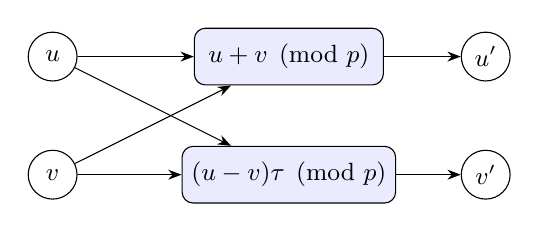
\begin{tikzpicture}[
    >=Stealth,
    val/.style={circle, draw, minimum size=0.62cm, inner sep=1pt, font=\small},
    op/.style={rounded corners, draw, fill=blue!8, minimum width=2.4cm,
              minimum height=0.72cm, align=center, font=\small},
]
  \node[val] (u) at (0, 0.75) {$u$};
  \node[val] (v) at (0, -0.75) {$v$};
  \node[op] (add) at (3.0, 0.75) {$u+v\pmod p$};
  \node[op] (sub) at (3.0, -0.75) {$(u-v)\tau\pmod p$};
  \node[val] (uo) at (5.5, 0.75) {$u'$};
  \node[val] (vo) at (5.5, -0.75) {$v'$};

  \draw[->] (u) -- (add);
  \draw[->] (v) -- (add);
  \draw[->] (u) -- (sub);
  \draw[->] (v) -- (sub);
  \draw[->] (add) -- (uo);
  \draw[->] (sub) -- (vo);
\end{tikzpicture}
\caption[Radix-2 NTT butterfly]{One forward DIF NTT butterfly.  A stage applies this fixed
  operation to $M/2$ independent input pairs, with position-dependent twiddles~$\tau$.}
\label{fig:ntt-butterfly}
\end{figure}

The regularity is as important as the asymptotic reduction.  Within a stage,
threads execute the same modular operations and differ principally in their
coefficient indices and twiddle values.  There is no data-dependent recursion,
and the power-of-two index relationships can be generated with shifts and
masks.

\subsubsection{Exact recovery from residues}

The inverse transform returns each convolution coefficient modulo~$p$.  A
residue $r$ has a unique centered interpretation
\begin{equation}
  \operatorname{center}(r)=
  \begin{cases}
    r, & 0\le r < p/2, \\
    r-p, & p/2 < r < p,
  \end{cases}
  \label{eq:ntt-centered-residue}
\end{equation}
provided that the true signed coefficient has absolute value below~$p/2$.
The base, transform ceiling, and fused product formulas are selected so that
the worst supported coefficient sum retains this headroom.  Consequently,
centered conversion recovers an integer coefficient, not an approximation to
one.  This exactness is the central reason for choosing an NTT over a
floating-point FFT in the reference engine.

\subsection{Why the NTT Maps Well to CUDA}
\label{subsec:ntt-gpu-mapping}

CUDA executes groups of threads in a SIMT hierarchy: lanes form warps, warps
form thread blocks, and a cooperative launch can synchronize the complete grid.
The official CUDA programming model describes both these group levels and the
residency requirement for grid-wide synchronization~\cite{NvidiaCudaProgrammingGuide}.
The NTT supplies useful work at each level.

\paragraph{Grid-level parallelism.}
Large butterfly stages address pairs that may be far apart.  The spectra reside
in global memory, and the cooperative grid distributes the transform work.
The release matrix schedule groups several butterfly stages into each phase;
grid-wide barriers separate phases that exchange data between blocks.  Local
stages reuse shared memory and warp registers.  The memory pattern remains
regular even when butterfly partners are distant.

\paragraph{Block-level locality.}
The release matrix schedule limits each shared-memory dimension to 2,048
coefficients in TwoWay mode.  FourWay mode permits up to 1,024 with 48~KiB of
dynamic shared memory, or 2,048 with at least 96~KiB.  The transform stages are
divided approximately evenly among dimensions, so actual dimensions can be
smaller: a $2^{16}$ transform uses two 256-coefficient dimensions.
One thread block stages the active streams for a local dimension.  Several
stages can then reuse those coefficients and cached twiddles without a
global-memory round trip.  Block barriers replace grid barriers inside the tile.  The same
shared arena is reused by forward, pointwise, inverse, and carry phases, so its
allocation cost is paid once per resident block rather than once per operator.

\paragraph{Warp-level exchange.}
When a complete 64-coefficient batch is available, the innermost five forward
stages, the pointwise products, and the first five inverse stages remain in
warp registers.  Shuffle operations exchange butterfly partners without a
block barrier.  Tiles that do not satisfy the eligibility conditions retain
the shared-memory path, preserving correctness for short or partial tails.

\paragraph{Concurrent streams.}
The orbit-only path transforms $x$ and $y$ in TwoWay mode.  Newton--Raphson
evaluation transforms $x$, $y$, $dx$, and $dy$ in FourWay mode.  All enabled
streams have the same $M$, roots, stage order, and dependency boundaries.
One thread can therefore apply a loaded twiddle to several streams before
moving to the next coefficient, and the additional derivative work does not
require a separate kernel schedule.

The match is not perfect.  One reference orbit supplies only one transform at
a time, so available grid parallelism is bounded by~$M$.  Shared memory and
registers constrain occupancy, modular multiplication has a dependency chain,
and large stages still require device-wide barriers.  The fused design is
therefore not based on an assumption that synchronization is free.  It reduces
the number of separately synchronized operators and places data at the
narrowest synchronization level that can legally contain each stage.

\subsection{High-Precision Representation and Alignment}
\label{subsec:hpfloat-model}

An \code{HpSharkFloat} value consists of a sign, a base-$2^{32}$ significand,
and an exponent.  If the significand limbs encode the nonnegative integer~$A$
and the sign bit encodes $s\in\{-1,1\}$, the represented value is
\begin{equation}
  v=sA2^e.
  \label{eq:hp-shark-value}
\end{equation}
The generated type fixes a compile-time storage bucket
\code{GlobalNumUint32}.  A runtime request selects an active limb count~$D$
greater than half the bucket size and at most its full size.  Arithmetic reads
the most significant $D$ limbs and ignores lower limbs, allowing one generated
specialization to serve a range of nearby precisions.

The NTT plan splits each active 32-bit limb into two base-$2^{16}$
coefficients.  Thus
\begin{equation}
  b=16,
  \qquad
  B=2^{16},
  \qquad
  L=2D.
  \label{eq:reference-b16-plan}
\end{equation}
The smaller coefficient base increases the number of transform elements but
leaves ample field headroom for the sum of many products and for the signs and
small integer factors in the fused recurrence.

Products and constants generally have different binary exponents.  The grid
leader therefore constructs a new \code{HpSharkReferenceIterationPlan} from the
current state before every attempted recurrence.  For each group of operands, it
chooses the least exponent among the nonzero values as the alignment origin.
An exponent difference is decomposed into a whole coefficient shift and a
residual shift:
\begin{equation}
  \Delta e = qb+r,
  \qquad
  q=\left\lfloor\frac{\Delta e}{b}\right\rfloor,
  \qquad
  0\le r<b.
  \label{eq:reference-alignment-split}
\end{equation}
The whole shift moves the coefficient support by~$q$ positions.  The residual
shift combines neighboring 16-bit halves while packing.  Alignment is thus
performed once in the input representation; the pointwise loop does not need
a frequency-dependent spectral shift.

For a nonzero component, the shift in~\eqref{eq:reference-alignment-split}
gives a last possible coefficient index
\begin{equation}
  k_{\max}=
  \begin{cases}
    q+L-1, & r=0, \\
    q+L, & r>0.
  \end{cases}
  \label{eq:reference-packed-support}
\end{equation}
The extra position in the second case holds bits carried out of the highest
16-bit coefficient by the residual shift.  Thus a real product involving both
$X$ and~$Y$ needs up to $2\max(k_X,k_Y)+1$ coefficients, while $X\star Y$
needs up to $k_X+k_Y+1$.  The same support calculation is applied to the
enabled derivative products.

The planner computes the last potentially nonzero coefficient for every
required product, including the derivative products, and rounds the largest
linear-convolution support up to a power of two.  The active length~$M$ is the
larger of that rounded length and the prepared minimum transform length, and
selects a cached plan.  The initial zero state still receives a plan.  A
zero state with no linear contribution takes the
\code{Zero} path, a state with only $c$ or the derivative's $+1$ takes the
\code{LinearOnly} path, and all nonlinear cases take the \code{Ntt} path.  A
required length beyond $2^{25}$ cannot be represented by the workspace; the
kernel reports an unknown status instead of allowing cyclic wraparound or an
out-of-bounds workspace access.

\subsection{Finite-Field and Transform Setup}
\label{subsec:reference-ntt-field}

The reference engine uses the Goldilocks prime
\begin{equation}
  p=2^{64}-2^{32}+1.
  \label{eq:reference-goldilocks-prime}
\end{equation}
Because
\begin{equation}
  p-1=2^{32}(2^{32}-1),
\end{equation}
the field contains power-of-two roots through order~$2^{32}$, comfortably
beyond the engine's $2^{25}$ workspace ceiling.  The setup kernel derives the
forward and inverse stage roots, fills the twiddle tables, computes the inverse
length, and marks each generated plan valid.  \code{ReferencePreparedTables}
owns these tables and the spectra, limb, magnitude, and carry workspaces.  The
tables are reused across all iterations and chunk invocations of a session.

Field products use Montgomery multiplication~\cite{Montgomery1985Modular}.
Write $R_{\mathrm M}=2^{64}$ for the Montgomery radix, distinct from the real
product $R$ below.  A field element $a$ in Montgomery form is
$\widetilde a=aR_{\mathrm M}\bmod p$, and a Montgomery product computes
\begin{equation}
  \operatorname{Mont}(\widetilde a,\widetilde c)
  =\widetilde a\widetilde c R_{\mathrm M}^{-1}
  =acR_{\mathrm M}\pmod p
\end{equation}
without integer division.  Additions and subtractions remain ordinary modular
operations.

The release path also absorbs transform normalization into packing.  For a
length-$M$ product, the prepared field value~$s$ satisfies
\begin{equation}
  s^2=(MR_{\mathrm M})^{-1}\pmod p.
  \label{eq:reference-input-scale}
\end{equation}
Packing actually multiplies each input coefficient by $sR_{\mathrm M}$,
represented in the code as \code{InputScaleR}.  If $\widehat a_k$ and
$\widehat c_k$ are the transforms of the unscaled inputs, linearity and one
pointwise Montgomery product give
\begin{align}
  \operatorname{NTT}(sR_{\mathrm M}a)_k
    &=sR_{\mathrm M}\widehat a_k, \\
  \operatorname{Mont}(sR_{\mathrm M}\widehat a_k,
                      sR_{\mathrm M}\widehat c_k)
    &=s^2R_{\mathrm M}\widehat a_k\widehat c_k.
\end{align}
The inverse stages omit their usual factor~$M^{-1}$, so the final coefficient
is $Ms^2R_{\mathrm M}h_j=h_j\pmod p$ by
\eqref{eq:reference-input-scale}.  It is already a standard residue ready for
centered conversion.  For an even number $t=\log_2M$ of stages,
$sR_{\mathrm M}=2^{32-t/2}\pmod p$, and packing uses a shift.  Odd stage
counts use a specialized multiply of a 16-bit coefficient by the prepared
constant.  No separate inverse-scale or Montgomery-exit pass is needed.

\subsection{The Fused Reference Recurrence}
\label{subsec:fused-ntt-reference-step}

Let $X$ and $Y$ denote the aligned coefficient polynomials for $x_n$ and
$y_n$.  Although~\eqref{eq:gpu-reference-components} is commonly written as
two squares and one product, the production pointwise stage uses the factored
real component
\begin{align}
  R &= (X+Y)\star(X-Y),
       \label{eq:fused-reference-real} \\
  I &= 2(X\star Y),
       \label{eq:fused-reference-imag}
\end{align}
where $\star$ denotes linear convolution.  These expressions equal
$X\star X-Y\star Y$ and $2X\star Y$ exactly but require only two nonlinear
products.  In the transform domain they become
\begin{align}
  \widehat R_k &= (\widehat X_k+\widehat Y_k)
                  (\widehat X_k-\widehat Y_k), \\
  \widehat I_k &= 2\widehat X_k\widehat Y_k.
  \label{eq:fused-reference-pointwise}
\end{align}
The signs of $x_n$ and $y_n$ have already been incorporated during packing.

The constants $c_x$ and $c_y$ are not transformed.  After the inverse NTT,
the signed gather inserts their significand bits at the offsets determined by
the iteration plan.  Interpreting $R$ and~$I$ at their planned product
exponents, carry propagation therefore implements the complete recurrence
\begin{align}
  x_{n+1} &= (x_n+y_n)(x_n-y_n)+c_x
           =x_n^2-y_n^2+c_x, \\
  y_{n+1} &= 2x_ny_n+c_y
\end{align}
without materializing normalized values for $R$ and~$I$ or launching a
standalone high-precision addition.

\subsubsection{Derivative products}
\label{subsec:fused-ntt-derivatives}

Newton--Raphson support also advances
\begin{equation}
  d_{n+1}=2z_nd_n+1,
  \qquad d_n=d_{x,n}+i d_{y,n}.
  \label{eq:fused-dzdc-complex}
\end{equation}
FourWay mode transforms the aligned derivative coefficient polynomials $D_x$
and $D_y$ with $X$ and~$Y$.  The pointwise center forms three products
\begin{align}
  P_1 &= X\star D_x, &
  P_2 &= Y\star D_y, &
  P_3 &= (X+Y)\star(D_x+D_y),
  \label{eq:fused-derivative-products}
\end{align}
The third product expands to
\begin{equation}
  P_3=P_1+X\star D_y+Y\star D_x+P_2,
\end{equation}
so subtracting $P_1$ and~$P_2$ isolates the two cross terms.  The nonlinear
coefficient polynomials are
\begin{align}
  2(P_1-P_2) &= 2(X\star D_x-Y\star D_y), \\
  2(P_3-P_1-P_2) &= 2(X\star D_y+Y\star D_x).
\end{align}
Interpreting these polynomials at their planned product exponent and inserting
the aligned constant gives the scalar recurrence
\begin{align}
  d_{x,n+1} &= 2(x_n d_{x,n}-y_n d_{y,n})+1, \\
  d_{y,n+1} &= 2(x_n d_{y,n}+y_n d_{x,n}).
  \label{eq:fused-derivative-reconstruction}
\end{align}
The derivative's $+1$ enters during signed gathering just as $c_x$ and~$c_y$
do; it is not an unshifted constant coefficient in the product polynomial.
The Gauss-style product identity reduces four real products to three and
shares every transform boundary with the orbit streams.

The second derivative
\begin{equation}
  q_{n+1}=2(d_n^2+z_nq_n)
\end{equation}
is used by the Feature Finder but does not join the high-precision FourWay NTT.
A leader thread updates its configured HDR representation from truncated orbit
and first-derivative values before the fused high-precision step.  The complete
Newton/Halley use of these values is described in
\cref{subsec:ff-inner-gpu}.

\subsubsection{Operation schedule}
\label{subsec:fused-ntt-operation-schedule}

\Cref{fig:ntt-pipeline} summarizes the release matrix schedule, selected for
$M>1024$ when checksum debugging is disabled.  Smaller transforms and checksum
debugging use the direct DIF/DIT schedule with tiles of at most 1,024
coefficients.  Matrix phases transform local dimensions and transpose data
between global buffers.  The center fuses its forward stages, pointwise
products, and inverse stages, keeping eligible innermost stages in warp
registers.  Red dashed boundaries indicate dependencies between grid-wide
phases; local stages synchronize only within the owning block or warp.

\begin{figure}[!htbp]
\centering
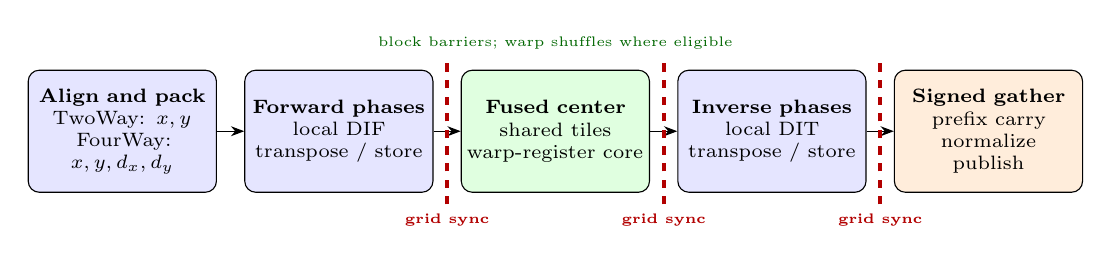
\begin{tikzpicture}[
    >=Stealth,
    phase/.style={draw, rounded corners, text width=2.25cm, inner xsep=0.07cm,
                  minimum height=1.55cm, align=center, font=\scriptsize},
    global/.style={phase, fill=blue!10},
    local/.style={phase, fill=green!12},
    carry/.style={phase, fill=orange!14},
    barrier/.style={draw, red!70!black, line width=1.4pt, dashed},
    barrlbl/.style={font=\tiny\bfseries, red!70!black},
]
  \node[global] (pack) at (0, 0)
    {\textbf{Align and pack}\\TwoWay: $x,y$\\FourWay: $x,y,d_x,d_y$};
  \node[global] (forward) at (2.75, 0)
    {\textbf{Forward phases}\\local DIF\\transpose / store};
  \node[local] (center) at (5.5, 0)
    {\textbf{Fused center}\\shared tiles\\warp-register core};
  \node[global] (inverse) at (8.25, 0)
    {\textbf{Inverse phases}\\local DIT\\transpose / store};
  \node[carry] (finish) at (11.0, 0)
    {\textbf{Signed gather}\\prefix carry\\normalize\\publish};

  \foreach \i/\j in {pack/forward, forward/center, center/inverse, inverse/finish}
    \draw[->] (\i) -- (\j);

  \foreach \x in {4.125, 6.875, 9.625} {
    \draw[barrier] (\x, -0.93) -- (\x, 0.93);
    \node[barrlbl] at (\x, -1.13) {grid sync};
  }

  \node[font=\tiny, green!40!black, align=center] at (5.5, 1.12)
    {block barriers; warp shuffles where eligible};
\end{tikzpicture}
\caption[GPU fused NTT schedule and synchronization hierarchy]{GPU fused NTT schedule for one
  iteration, shown as conceptual phases rather than a fixed barrier count.
  Packing is fused into the first active transform phase.  Forward and inverse
  phases outside the center may repeat or be absent, depending on the dimension
  count.  FourWay mode widens the streams and products and can change that count.}
\label{fig:ntt-pipeline}
\end{figure}

In the matrix path, one nonlinear iteration proceeds as follows:

\begin{enumerate}
  \item The grid leader inspects the normalized state, builds the alignment and
        support plan, and publishes its kind, active~$M$, offsets, and flags.
  \item Threads pack signed base-$2^{16}$ coefficients at their aligned
        positions and apply the input scale from
        ~\eqref{eq:reference-input-scale}.  Packing is fused into the first
        forward matrix phase, or into the center for a single-dimension plan.
  \item Forward matrix phases, when needed, transform local dimensions and
        transpose their outputs for the next phase, with grid synchronization
        between phases.
  \item Each block loads a shared-memory center dimension, completes the small
        forward stages, evaluates~\eqref{eq:fused-reference-pointwise} and, when enabled,
        ~\eqref{eq:fused-derivative-products}, and begins the inverse DIT.
  \item Inverse matrix phases, when needed, reverse the dimension traversal.
        The completed inverse returns natural-order coefficients as standard
        residues in global memory.
  \item The signed gather centers residues, incorporates $c_x$, $c_y$, and the
        derivative's $+1$, and constructs carry transfer functions.
  \item A packed prefix operation resolves the carry chains.  Magnitude
        extraction and normalization publish the next orbit and derivative
        states.
  \item If another iteration is requested, the next loop entry records the
        current low-precision orbit value and checks periodicity and escape
        when enabled.  A bounded batch is returned to the host after the launch.
\end{enumerate}

\subsubsection{DIF/DIT ordering and implicit permutation}

In the direct radix-2 schedule, the forward DIF transform consumes natural-order
coefficients and leaves its spectrum in bit-reversed order.  Pointwise products do not care about that
permutation as long as every stream uses the same order.  The inverse DIT
transform consumes the bit-reversed spectra and emits natural-order
coefficients.  Pairing the two variants therefore avoids a separate bit-reversal
kernel and its global reads, writes, and synchronization.  The matrix schedule
also transposes between dimensions, but applies matching permutations to every
stream and pairs its forward and inverse layouts.  Avoiding a standalone
bit-reversal pass does not eliminate those transposes.

The fused center exploits the same pairing more aggressively.  It completes
the small forward stages, evaluates the pointwise recurrence, and starts the
small inverse stages while a tile is resident.  The data need not be written to
a standalone \emph{forward result} buffer and then loaded by an unrelated
multiply operator.  This is the central meaning of \emph{fused} in v2.

\subsection{Signed Carry, Normalization, and Exactness}
\label{subsec:fused-ntt-carry}
\label{sec:hp-add}

Three independent conditions make the modular result an exact positional
result:

\begin{enumerate}
  \item The active~$M$ contains the complete shifted linear-convolution support,
        so no nonzero coefficient wraps around $x^M-1$.
  \item The absolute coefficient bound for every enabled orbit and derivative
        combination is below $p/2$, so
        ~\eqref{eq:ntt-centered-residue} recovers the unique signed integer.
  \item Carry propagation includes every nonlinear and aligned linear
        contribution before normalization truncates the result to its storage
        bucket; subsequent arithmetic reads the selected $D$ most significant limbs.
\end{enumerate}

The coefficient bound can be made explicit for the nonlinear terms.  Each
unscaled aligned input coefficient has absolute value at most $B-1$, and each
linear convolution coefficient has at most $M$ contributing pairs.  The factored real
product has bound $4M(B-1)^2$, while $2X\star Y$ has bound $2M(B-1)^2$.
Writing $[P]_j$ for coefficient~$j$ of a polynomial~$P$, the derivative products
satisfy $|[P_1]_j|,|[P_2]_j|\le M(B-1)^2$ and
$|[P_3]_j|\le 4M(B-1)^2$.  Consequently, the largest
conservative bound among the reconstructed nonlinear coefficients is
\begin{equation}
  |[2(P_3-P_1-P_2)]_j|
  \le 12M(B-1)^2
  \le 12\cdot 2^{25}(2^{16}-1)^2
  < \frac{p-1}{2}.
  \label{eq:reference-centered-headroom}
\end{equation}
The aligned constants are added after centered recovery, so they do not
consume this modular headroom.  Exactness here means exact coefficients for
the finite-precision inputs before the final significand truncation; it does
not make the entire iterated orbit exact over real numbers.

After centering, adjacent base-$2^{16}$ coefficients contribute to signed
base-$2^{32}$ limbs.  The fused B16 gather performs that conversion in the same
warp that constructs the carry metadata; release builds do not need to
materialize and reread four complete signed-limb arrays.  Debug builds may
materialize them so that the host and device checkpoints remain directly
comparable.

A carry chain is sequential if represented only as individual carry values.
It becomes parallel once a limb interval is represented as a transfer function
from its bounded incoming carry to its outgoing carry.  Function composition is
associative, so warp scans combine thread summaries, a block scan combines warp
summaries, and decoupled look-back resolves preceding block partitions.  The
method follows the parallel-prefix framework of Blelloch~\cite{Blelloch1990PrefixSums}
and the single-pass decoupled-look-back construction of Merrill and
Garland~\cite{merrill2016single}.

Concretely, for signed limb contribution $\ell_j$, incoming carry $\kappa_j$,
and base $Q=2^{32}$, the emitted digit and outgoing carry satisfy
\begin{equation}
  d_j=(\ell_j+\kappa_j)\bmod Q,
  \qquad
  \kappa_{j+1}=\frac{\ell_j+\kappa_j-d_j}{Q},
  \qquad 0\le d_j<Q.
  \label{eq:reference-signed-carry}
\end{equation}
Each limb therefore defines a small function
$\kappa_j\mapsto\kappa_{j+1}$.  Prefix composition finds every incoming
carry, after which the digits can be emitted independently, including when a
convolution coefficient or a linear contribution is negative.

The implementation packs the transfer functions for real, imaginary,
derivative-real, and derivative-imaginary streams into one 32-bit word in
FourWay mode.  A single composition instruction sequence therefore advances
four logically independent carry chains through the same scan topology.  After
the incoming carries are known, threads emit the final 32-bit digits in
parallel.

Normalization determines the sign, extracts the magnitude, finds the highest
nonzero digit, writes the fixed \code{GlobalNumUint32}-limb storage bucket, and
adjusts the exponent to preserve the retained bits' positional weights.
Subsequent arithmetic consumes only the most significant $D$ limbs of that
normalized bucket.  The next
iteration cannot begin from the inverse spectra alone: its alignment plan needs
this normalized sign, exponent, and significand.  Returning to
\code{HpSharkFloat} form is therefore a semantic dependency, not merely a
storage-format preference.

\subsection{Persistent Kernel and Host Lifecycle}
\label{subsec:ref-orbit-architecture}

Setup and execution have separate lifetimes.  The host selects a generated
storage family, chooses the active limb count, and constructs
\code{ReferencePreparedTables}.  Setup allocates one contiguous workspace,
assigns its spectrum and scratch regions, prepares plan descriptors from the
selected minimum through the selected maximum stage (stage~25 by default),
and launches the setup kernel to
generate their roots and twiddles.

\code{GpuOrbitSession} then owns the result descriptor and the CUDA stream for
one reference calculation.  Repeated \code{InvokeChunk} calls launch the
persistent recurrence for a requested number of iterations.  The production
callers limit each request to \code{MaxOutputIters}=1024 iterations, matching
the orbit-output capacity; \code{InvokeChunk} forwards the requested count.
The chunk limit bounds host transfer size and creates regular opportunities for cancellation and progress
handling without introducing a kernel launch for every recurrence.

Inside a launch, \code{HpSharkReferenceGpuLoop} obtains a cooperative
\code{grid\_group}.  Grid synchronization is required because a large NTT stage
can exchange data produced by different blocks.  A cooperative launch also
constrains the grid to blocks that can be resident together; launch selection
must therefore respect registers, dynamic shared memory, and the device's
cooperative occupancy.  The persistent organization amortizes launch overhead
and preserves the workspace across many sequential iterations, but it does not
remove the cost of the necessary barriers.

The generated CUDA translation units instantiate four families:
\code{HpSharkFloat\_\allowbreak Conversions}, \code{HpShark\allowbreak Reference},
\code{ReferenceGpu\allowbreak Loop}, and \code{SharkNTT\_\allowbreak Primitives}.  They provide
host/device conversion, lifecycle operations, the persistent recurrence, and
the Montgomery primitives shared with the host correctness model.  Explicit
instantiation keeps the supported precision families finite and makes their
workspace limits compile-time properties.

\subsection{Periodicity, Escape, and Resume Semantics}
\label{subsec:fused-ntt-periodicity}

When periodicity checking is enabled, the grid leader converts the current
high-precision orbit state to HDR values and evaluates the reduced-precision
criterion described in \cref{sec:hp-periodicity}.  Its derivative tracker is
also HDR, distinct from the FourWay high-precision derivative streams.
A continuing state allows the iteration plan to be built.  Escape, a positive periodicity result,
or an unrepresentable plan prevents the grid from entering another collective
phase.  This ordering is important: all threads must agree on whether they will
reach a cooperative barrier.

At loop entry, the ordinary reference path stores a low-precision sample of
the current $z_n$ and tests it before attempting the next recurrence.  The
leader increments the output count after a completed step, or when the
periodicity or escape check terminates on that sampled value.  The
next pass, if any, tests the newly published $z_{n+1}$.  The
Feature Finder instead returns the high-precision endpoint and derivative
state after its requested period.  Both clients use the same fused arithmetic
engine and differ in how they consume the results.

Ordinary reference construction starts the GPU state at $z=c$, with its HDR
derivative tracker initialized to one; the host supplies the preceding zero
orbit entry.  Feature Finder evaluation instead treats \code{startIter}=0 as
fresh initialization with $z_0=d_0=q_0=0$.  A positive \code{startIter} consumes
the supplied orbit and derivative values and continues from that checkpoint.  Abort and progress callbacks are
polled at bounded host-visible intervals without changing this contract.

\subsection{Checksum-Guided Host--Device Validation}
\label{sec:checksums}

Exact arithmetic makes bitwise stage comparison possible.  Debug builds can
record checksums after aligned packing, forward transforms, pointwise products,
inverse transforms, signed gathering, carry, and normalization.  The retained
\code{ReferenceReferenceOrbit2} CPU oracle executes the same plan and records
the corresponding host states.  \code{ChecksumsCheck} compares states by
purpose and call index, localizing a disagreement to a pipeline boundary
without retaining the obsolete v1 arithmetic operators.

The tests cover more than a forward/inverse round trip.  They compare orbit
outputs against MPIR, exercise exponent gaps and transform-length changes,
cover TwoWay and FourWay modes, verify checkpoint continuation, and run long
Newton sequences.  This breadth is required because an error in a late NTT
stage, a tail tile, or carry look-back can survive a short smoke test and become
visible only after many recurrence steps.

\subsection{Design Tradeoffs and Scope}
\label{subsec:fused-ntt-tradeoffs}

The fused v2 design is optimized for the regime in which high-precision
multiplication dominates reference construction.  Its main strengths are exact
field arithmetic, regular coefficient-level parallelism, transform reuse across
multiple streams, elimination of explicit bit reversal, and the absence of
normalized product temporaries.  Its costs are root and workspace preparation,
global barriers for large stages, modular-multiply latency, and occupancy
pressure from registers and shared memory.  A shorter operand may therefore be
better served by simpler arithmetic in another backend even though the NTT has
better asymptotic scaling.

Fusion also has a boundary.  Algebraic additions and derivative products can be
placed inside the shared transform and carry schedule, but independent orbit
iterations cannot be overlapped without changing the recurrence.  The inverse
transform, carry, and normalization cannot be moved to the end of the entire
orbit because the next iteration needs their result.  The implementation
concentrates on removing avoidable boundaries while retaining the mathematical
ones.

The application exposes one production selector for this engine.  The portable
menu labels it \emph{GPU-Accelerated Reference Orbit}, the Feature Finder labels
its backend \emph{NR Inner Loop: GPU}, and the CLI accepts \code{GPU}.
Reference-orbit rendering uses \code{GpuOrbitSession}; the Feature Finder calls
\code{EvaluateCriticalOrbitAnd\allowbreak Derivs\_\allowbreak GPU} through
\code{OrbitEndpoint\allowbreak Evaluator}.  The CUDA test harness retains
\code{Operator::\allowbreak ReferenceOrbit2} only as the established correctness-test
identity.  Production setup, execution, and shutdown use the unnumbered
\code{PrepareHpShark\allowbreak ReferenceTables},
\code{InvokeHpShark\allowbreak ReferenceKernel}, and
\code{ShutdownHpShark\allowbreak ReferenceKernel} interfaces.

\input{FractalShark-18-FeatureFinder}

% ============================================================
% Part III: Supporting Infrastructure
% ============================================================
\part{Supporting Infrastructure}

\input{FractalShark-19-RenderPipeline}
\input{FractalShark-22-MemorySystem}

% ============================================================
% Part IV: Further Techniques
% ============================================================
\part{Further Techniques}

\input{FractalShark-23-FutureDirections}

% ============================================================
% Conclusion
% ============================================================
\input{FractalShark-24-Conclusion}

% ============================================================
% Appendices
% ============================================================
\appendix
\part{Appendices}

\section{User Documentation}
\label{sec:user-documentation}

This appendix collects the user-facing guides for the interactive application,
keyboard-driven workflows, automatic zoom modes, and headless renderers.

\subsection{User Interface and Popup Menu Guide}
\label{sec:ui-popup-menu}

\FractalShark{} can be driven \emph{entirely} from the keyboard and mouse, with the
right-click popup menu acting as the primary discovery and configuration
surface.  Day-to-day navigation (zooming, recentering, going back, iteration
adjustment, palette cycling, and several recomputation paths) is also exposed
through single-key shortcuts, so common workflows do not require opening the
menu.

The popup menu is context-sensitive and rebuilt dynamically each time it is
shown. Both front ends derive checked, enabled, and disabled states from the
same portable menu-state implementation and current rendering state. The menu
can be invoked by mouse (\textbf{right-click}) on both
platforms. The Win32 GUI also supports the standard keyboard context-menu
invocation (\textbf{Shift+F10} / \textbf{Menu} key).

\subsubsection{Basic Interaction}

On startup, \FractalShark{} displays a brief splash screen (randomly chosen
from a set of built-in images) while initializing the renderer.

The most common interactions are:
\begin{itemize}
  \item \textbf{Right-click}: Open the popup menu at the mouse cursor.
  \item \textbf{Left-click and drag}: Zoom into a rectangular region.
        By default the zoom rectangle preserves the window aspect ratio;
        holding \code{Shift} while dragging allows a free-form
        (non-square) selection.
  \item \textbf{Mouse wheel}: Scroll forward to zoom in at the cursor;
        scroll backward to zoom out from the center.
  \item \textbf{Keyboard shortcuts}:
    \begin{itemize}
      \item \code{z}: Zoom in at the mouse cursor.
      \item \code{Shift+Z}: Zoom out slightly.
      \item \code{b}: Return to the previous view.
      \item \code{- / =}: Decrease or increase the iteration limit.
    \end{itemize}
\end{itemize}

Resizing the window automatically resets the renderer dimensions and triggers
a recalculation of the fractal to match the new window size.

\paragraph{Linux graphical front end.}
Version~0.53 is the first release with experimental Linux support. The native
Linux application is \code{FractalSharkGuiLinux}. It uses an X11 window and
native hierarchical popup menu, presents rendered frames through OpenGL, and
uses Dear~ImGui for help, file-selection, saved-location, and manual
location-entry dialogs. It supports the primary mouse and keyboard navigation
paths, fullscreen and square-fullscreen modes, the shared render and
perturbation commands, automatic zoom and feature finding, clipboard export,
and the save/load workflows described below. The application requires a
working X display and GLX/OpenGL implementation. GPU algorithms additionally
require supported NVIDIA CUDA hardware; CPU algorithms remain available when
GPU rendering is bypassed.

Most commands have the same meaning on Windows and Linux because both front
ends dispatch through the shared command catalog and evaluate state through the
same portable implementation.

\subsubsection{Menu Structure and Behavior}

The popup menu is organized into logical groups and submenus. Items fall into
three distinct behavioral categories:

\begin{description}
  \item[Radio groups] Mutually exclusive choices where exactly one option is
  active at a time (for example, selecting a render algorithm or GPU antialiasing level).
  \item[Toggles] Binary on/off options that switch between two states each time
  they are selected (for example, toggling repainting or full-screen mode).
  \item[Commands] Immediate actions that execute when selected and do not
  maintain a checked state.
\end{description}

Radio groups reflect the configuration in use, with the currently active option
checked. Selecting a different option automatically deselects the previous
choice and triggers any necessary reconfiguration.

\subsubsection{Top-Level Menu}

\begin{itemize}
  \item \emph{Show Help} (command): Displays an on-screen help dialog summarizing keyboard shortcuts.

  \item \emph{Navigate} (submenu):
    \begin{itemize}
      \item \emph{Back} (command): Navigate back to the previous view in history.
      \item \emph{Center View Here} (command): Centers the current view on the
      point under the cursor.
      \item \emph{Zoom In Here} (command): Zooms in toward the point under the cursor.
      \item \emph{Zoom Out} (command): Zooms out from the current view.
      \item \emph{Autozoom Default} (command): See \cref{par:autozoom} for details.
      \item \emph{Autozoom Max} (command): Autozoom using the ``Max'' heuristic,
      which zooms by a factor of~32 each step.  See \cref{par:autozoom} for details.
      \item \emph{Autozoom Filament Tip} (\code{S}, i.e.\ \code{Shift+s}) (command): Autozoom using the
      ``FilamentTip'' heuristic.
      \item \emph{Feature Finder} (submenu): Locates nearby mini-Mandelbrot
      nuclei (periodic points) using Newton's method and optionally zooms to
      them.  Three evaluation back-ends are available, each in a single-point
      and a whole-screen scan variant.  See
      \cref{sec:feature-finder} for the underlying algorithm.
        \begin{itemize}
          \item \emph{Direct} (\code{n}) (command): Runs the feature finder at
          the mouse cursor using direct iteration.  Best for shallow zooms where
          no perturbation data is needed.
          \item \emph{DirectScan} (\code{N}) (command): Runs direct-iteration
          feature finding on a $12\times12$ grid across the entire viewport,
          locating multiple features at once.
          \item \emph{PT} (\code{m}) (command): Runs the feature finder at the
          mouse cursor using perturbation theory (\cref{sec:perturbation-concept}).
          Requires a reference orbit and works at deeper zooms than Direct.
          \item \emph{PTScan} (\code{M}) (command): Runs perturbation-theory
          feature finding on a $12\times12$ grid across the viewport.
          \item \emph{LA} (\code{,}) (command): Runs the feature finder at the
          mouse cursor using linear approximation (\cref{sec:la-v2-perturb}).
          Works at extreme zoom depths where PT alone would be too slow.
          \item \emph{LAScan} (\code{<}) (command): Runs linear-approximation
          feature finding on a $12\times12$ grid across the viewport.
          \item \emph{Zoom to Found Feature} (\code{.}) (command): Zooms into
          the most recently found feature.  If the feature has only been located
          at low precision, a high-precision GMP refinement pass is performed
          automatically before zooming.
          \item \emph{Clear All Found Features} (\code{>}) (command): Removes
          all found-feature overlays (lines and circles drawn on the fractal).
          \item \emph{Resume NR Refinement} (command): Resumes
          Newton--Raphson precision refinement from the most recent checkpoint,
          useful when a prior refinement was interrupted or when additional
          precision is desired.
          \item \emph{NR Inner Loop: GPU / CPU} (radio): Selects
          whether the Newton--Raphson inner loop (iterating the orbit and
          derivatives for $p$~steps) executes on the GPU via
          \code{HpSharkFloat} or falls back to CPU-based MPIR arithmetic.
        \end{itemize}
      When a feature is found, a line is drawn from the search origin to the
      detected nucleus, making its location visible.  Scan modes are useful for
      surveying an entire view at a glance; single-point modes are faster and
      target the area near the cursor.
    \end{itemize}

  \item \emph{Built-In Views} (submenu): Loads a predefined view/location used
  for demonstrations, debugging, or performance testing.  Up to 32 views are
  defined in the source (\code{FractalViewPresets.cpp}).
    \begin{itemize}
      \item \emph{Help} (command): Pops up a message box that simply says this
      submenu contains built-in test views.
      \item \emph{Standard View} (command): Loads the default starting view: the
      classic Mandelbrot.
      \item \emph{\#1 -- \#32} (commands): Loads a specific predefined
      test view. Many entries encode expected precision limits, kernel behavior,
      or known failure cases in their label text.  Several views require intense
      computation and take a long time to render.  View \#27, for example, is a
      period ~28 billion point that takes hours to render and requires reference
      compression even with 128GB of RAM.  Exercise caution when selecting deep-zoom
      views, as they may cause long delays or high memory usage.

    \end{itemize}
    When reference orbits or Imagina-format orbit files are loaded, additional
    dynamic view entries may appear in the menu below the built-in presets.
    These entries correspond to the loaded data and are removed when the orbit
    state is cleared.

  \item \emph{Recalculate, Reuse Reference} (command): Forces an immediate
  re-render using the current settings, reusing the existing reference orbit if
  possible.  See \cref{subsec:recalculation-commands} for details.

  \item \emph{Toggle Repainting}: Enables or disables progressive
  repainting while a render is in progress. When disabled, no recalculation
  takes place on window resize or related, which can be helpful when a new
  window size is desired without triggering a re-render.
  \item \emph{Toggle Window Size}: Toggles between windowed and
  full-screen behavior.  The window stays at the same aspect ratio by default.
  \item \emph{Toggle Window Size (Square)}: Toggles an alternate sizing
  mode constrained to a square aspect ratio.
  \item \emph{Minimize Window} (command): Minimizes the application window.

  \item \emph{Antialiasing} (radio group submenu): Selects the antialiasing
  level used for rendering.
    \begin{itemize}
      \item \emph{1x (fast)}
      \item \emph{4x}
      \item \emph{9x}
      \item \emph{16x (better quality)}
    \end{itemize}

  Note that antialiasing as used here is not traditional GPU antialiasing.
  Instead, 4, 9, or 16 samples are explicitly computed per pixel and averaged
  together either on the CPU or GPU.  This approach is known as
  \emph{supersampling} and produces high-quality results at the cost of
  increased computation time and memory usage.  It's a naive approach---in
  principle, more sophisticated techniques could be implemented in the future,
  such as edge-aware sampling or adaptive sampling.

  \item \emph{Choose Render Algorithm} (radio group submenu): Selects the core
  Mandelbrot rendering strategy. This submenu is a radio group: selecting one algorithm
  automatically deselects the others. Available choices may include CPU-based
  reference and linear-approximation renderers, multiple CUDA-based GPU
  renderers, and high-dynamic-range and experimental kernels. On systems without
  a working CUDA setup, CPU renderers can be selected as a fallback. In the
  event of a CUDA initialization failure, switching to a CPU algorithm followed
  by a recalculation may restore a usable image.

  Algorithm names follow a systematic convention:
  \begin{description}
    \item[\textrm{N}x\textrm{BB}] Precision type: \emph{N} is the number of
    components and \emph{BB} is the component bit-width.
    \code{1x32}~=~single float, \code{2x32}~=~double-float
    (\cref{subsec:ep-dblflt}), \code{1x64}~=~double,
    \code{2x64}~=~double-double, \code{4x32}/\code{4x64}~=~quad
    types (\cref{subsec:ep-higher-prec}).
    \item[HDR] High Dynamic Range: the type is wrapped in
    \code{HDRFloat} (\cref{sec:hdr-float}) for extended exponent range,
    required at deep zooms.
    \item[RC] Reference Compression: the reference orbit is stored in
    compressed form (\cref{sec:ref-compression-zhuoran}).
    \item[Perturbation / Perturb] Per-pixel perturbation from a
    reference orbit (\cref{sec:perturbation-concept}).
    \item[BLA] Bilinear Approximation v1 (\cref{sec:bilinear-approx}).
    \item[LA~v2] Linear Approximation v2 (\cref{sec:la-v2-perturb}),
    the primary deep-zoom rendering path.
    \item[Scaled] An alternative perturbation formulation using a
    rescaled delta; partially broken.
    \item[LA only / Perturb only] Testing modes that run only one
    stage of the pipeline in isolation.
  \end{description}
  For example, \emph{HDRx2x32 GPU -- RC LA~v2} means: GPU kernel using
  a 2$\times$32-bit (double-float) type wrapped in HDR, with reference
  compression and the LA~v2 full pipeline.  Individual algorithm entries
  below are not further annotated because their names are
  self-documenting given this convention.

    \begin{itemize}
      \item \emph{Help} (command): Displays help for algorithm selection and
      related concepts (e.g., what LA~v2 (\cref{sec:la-v2-perturb}), BLA
      (\cref{sec:bilinear-approx}), perturbation (\cref{sec:perturbation-concept}),
      and reference compression (\cref{subsec:ref-orbit-compression-reuse}) mean,
      and when to use each).

      \item \emph{Auto (Default)} (radio): Automatically selects the
      default/recommended renderer.  Recommended.

      \emph{Note}: this option exhibits potentially-confusing behavior.  When
      selected, it does not lock in a specific algorithm; rather, it allows the
      system to choose the most appropriate algorithm based on current view
      parameters. The radio button for "Auto" will not be checked; instead, the
      actual algorithm in use will be checked.  Thus, selecting \emph{Auto} may
      appear to have no effect, but navigating the submenus reveals that the
      algorithm currently in use is checked.  This design allows users to see
      what algorithm is active.

      When GPU rendering is active, four algorithms are eligible for automatic
      selection:
      \begin{itemize}
        \item \emph{1x32 GPU}: The default low-zoom GPU renderer.  No
              perturbation or linear approximation is used.
        \item \emph{1x32 GPU -- Perturb only}: The default
              perturbation-only GPU renderer (\cref{sec:perturb-only}) for
              moderate zooms uses perturbation but no linear approximation.
        \item \emph{1x32 GPU -- LA~v2}: A bit deeper, no high-dynamic range
              floats but does use linear-approximation renderer and
              perturbation.
        \item \emph{HDRx32 GPU -- LA~v2}: Arbitrary depth (\cref{sec:la-v2-perturb,sec:hdr-float}), combines all known
              algorithmic optimizations.  This one can result in rendering
              artifacts at some deep locations due to numeric precision
              limitations.  ``Auto'' mode cannot detect this, so if artifacts appear, try
              HDRx2x32 or HDRx64 variants instead.  View \#26 is an example of a
              point that fails with HDRx32 but works correctly with HDRx64.

              See \cref{fig:auto-renderer-artifact} for an example of
              artifacts that can arise when using HDRx32 at extreme depths.
      \end{itemize}
      If GPU rendering is bypassed or unavailable, \emph{Auto} follows the same
      zoom-factor tiering shape with CPU renderers: \emph{1x64 CPU} below
      $10^9$, \emph{1x64 CPU -- Perturbation BLA} below $10^{34}$, and
      \emph{HDRx64 CPU -- Perturbation LA~v2} at deeper zooms.

      \item \emph{LA Parameters} (submenu): Controls linear-approximation (LA) configuration and tuning.
        \begin{itemize}
          \item \emph{Multithreaded (Default)} (radio): Uses multithreaded LA processing.
          \item \emph{Single Threaded} (radio): Uses single-threaded LA processing.
          \item \emph{Max Accuracy (Default)} (command): Resets all LA threshold
          and period-detection exponents to their conservative defaults.  Produces the
          most accurate linear approximation at the cost of longer computation.
          \item \emph{Max Performance (Accuracy Loss)} (command): Increases the LA
          threshold scale exponents by~12 relative to defaults, allowing the
          approximation to accept looser tolerances.  This speeds up LA computation
          but may introduce visible artifacts at some locations.
          \item \emph{Min Memory} (command): Increases the period-detection threshold
          exponents by~3, causing the period detector to accept matches more eagerly.
          This setting reduces the number of stored LA stages and lowers memory consumption.
        \end{itemize}

      \item \emph{CPU-Only} (submenu): CPU renderers and CPU-driven perturbation variants.
        \begin{itemize}
          \item \emph{Very High Precision CPU} (radio)
          \item \emph{1x64 CPU} (radio)
          \item \emph{HDRx32 CPU} (radio)
          \item \emph{HDRx64 CPU} (radio)

          \item \emph{1x64 CPU -- Perturbation BLA} (radio)
          \item \emph{HDRx32 CPU -- Perturbation BLA} (radio)
          \item \emph{HDRx64 CPU -- Perturbation BLA} (radio)

          \item \emph{HDRx32 CPU -- Perturbation LA~v2} (radio)
          \item \emph{HDRx64 CPU -- Perturbation LA~v2} (radio)
          \item \emph{HDRx32 RC CPU -- Perturbation LA~v2} (radio)
          \item \emph{HDRx64 RC CPU -- Perturbation LA~v2} (radio)
        \end{itemize}

      \item \emph{Low-Zoom Depth} (submenu): GPU renderers intended for relatively modest zoom depths and lower precision requirements.
        \begin{itemize}
          \item \emph{Iteration Precision} (radio group submenu): Controls a
          rendering speed/quality trade-off for low-zoom GPU paths.  The
          internal multiplier (1, 4, 8, or~16) scales the iteration step size:
          higher multipliers compute faster but with lower fidelity.
            \begin{itemize}
              \item \emph{4x (fast)} (radio): Multiplier~16 (fastest, lowest quality).
              \item \emph{3x} (radio): Multiplier~8.
              \item \emph{2x} (radio): Multiplier~4.
              \item \emph{1x (better quality)} (radio): Multiplier~1 (slowest, highest quality).
            \end{itemize}

          \item \emph{1x32 GPU} (radio)
          \item \emph{2x32 GPU} (radio)
          \item \emph{4x32 GPU} (radio)
          \item \emph{1x64 GPU} (radio)
          \item \emph{2x64 GPU} (radio)
          \item \emph{4x64 GPU} (radio)
          \item \emph{HDRx32 GPU} (radio)
        \end{itemize}

      \item \emph{Scaled} (submenu): Perturbation renderers using a scaled formulation.
        \begin{itemize}
          \item \emph{1x32 GPU -- Perturbation Scaled} (radio)
          \item \emph{2x32 GPU -- Perturbation Scaled (broken)} (radio)
          \item \emph{HDRx32 GPU -- Perturbation Scaled} (radio)
        \end{itemize}

      \item \emph{Bilinear Approximation V1} (submenu): Perturbation renderers using the original bilinear approximation approach.
        \begin{itemize}
          \item \emph{1x64 GPU -- Perturbation BLA} (radio)
          \item \emph{HDRx32 GPU -- Perturbation BLA} (radio)
          \item \emph{HDRx64 GPU -- Perturbation BLA} (radio)
        \end{itemize}

      \item \emph{LA Only (for testing)} (submenu): Test configurations that run only the linear-approximation portion of the pipeline.
        \begin{itemize}
          \item \emph{1x32 GPU -- LA~v2 -- LA only} (radio)
          \item \emph{2x32 GPU -- LA~v2 -- LA only} (radio)
          \item \emph{1x64 GPU -- LA~v2 -- LA only} (radio)
          \item \emph{HDRx32 GPU -- LA~v2 -- LA only} (radio)
          \item \emph{HDRx2x32 GPU -- LA~v2 -- LA only} (radio)
          \item \emph{HDRx64 GPU -- LA~v2 -- LA only} (radio)
        \end{itemize}

      \item \emph{Perturbation Only} (submenu): Test configurations that run only the perturbation portion of the pipeline.
        \begin{itemize}
          \item \emph{1x32 GPU -- Perturb only} (radio)
          \item \emph{2x32 GPU -- Perturb only} (radio)
          \item \emph{1x64 GPU -- Perturb only} (radio)
          \item \emph{HDRx32 GPU -- Perturb only} (radio)
          \item \emph{HDRx2x32 GPU -- Perturb only} (radio)
          \item \emph{HDRx64 GPU -- Perturb only} (radio)
        \end{itemize}

      \item \emph{Reference Compression} (submenu): Algorithms using reference-orbit compression as part of the perturbation pipeline.
        \begin{itemize}
          \item \emph{1x32 GPU -- RC LA~v2} (radio)
          \item \emph{2x32 GPU -- RC LA~v2} (radio)
          \item \emph{1x64 GPU -- RC LA~v2} (radio)
          \item \emph{HDRx32 GPU -- RC LA~v2} (radio)
          \item \emph{HDRx2x32 GPU -- RC LA~v2} (radio)
          \item \emph{HDRx64 GPU -- RC LA~v2} (radio)

          \item \emph{Perturbation Only} (submenu): Reference-compressed perturbation-only variants.
            \begin{itemize}
              \item \emph{1x32 GPU -- RC Perturb Only} (radio)
              \item \emph{2x32 GPU -- RC Perturb Only} (radio)
              \item \emph{1x64 GPU -- RC Perturb Only} (radio)
              \item \emph{HDRx32 GPU -- RC Perturb Only} (radio)
              \item \emph{HDRx2x32 GPU -- RC Perturb Only} (radio)
              \item \emph{HDRx64 GPU -- RC Perturb Only} (radio)
            \end{itemize}

          \item \emph{LA Only} (submenu): Reference-compressed LA-only variants.
            \begin{itemize}
              \item \emph{1x32 GPU -- RC LA~v2 -- LA only} (radio)
              \item \emph{2x32 GPU -- RC LA~v2 -- LA only} (radio)
              \item \emph{1x64 GPU -- RC LA~v2 -- LA only} (radio)
              \item \emph{HDRx32 GPU -- RC LA~v2 -- LA only} (radio)
              \item \emph{HDRx2x32 GPU -- RC LA~v2 -- LA only} (radio)
              \item \emph{HDRx64 GPU -- RC LA~v2 -- LA only} (radio)
            \end{itemize}
        \end{itemize}

      \item \emph{LA~v2 (Full Pipeline)} (radio entries): Main LA~v2 renderers combining LA, perturbation, and reference handling.
        \begin{itemize}
          \item \emph{1x32 GPU -- LA~v2} (radio)
          \item \emph{2x32 GPU -- LA~v2} (radio)
          \item \emph{1x64 GPU -- LA~v2} (radio)
          \item \emph{HDRx32 GPU -- LA~v2} (radio)
          \item \emph{HDRx2x32 GPU -- LA~v2} (radio)
          \item \emph{HDRx64 GPU -- LA~v2} (radio)
        \end{itemize}

      \item \emph{Tests} (submenu): Development and diagnostic test actions.
        \begin{itemize}
          \item \emph{Run Basic Test (saves files in local dir)} (command)
          \item \emph{Run View \#27 test} (command)
        \end{itemize}

    \end{itemize}

  \item \emph{Iterations} (submenu): Adjusts the iteration limit and iteration counter width.
    \begin{itemize}
      \item \emph{Default Iterations} (command): Resets iteration count to defaults.
      \item \emph{+1.5x} (command): Multiplies iteration limit by 1.5.
      \item \emph{+6x} (command): Multiplies iteration limit by 6.
      \item \emph{+24x} (command): Multiplies iteration limit by 24.
      \item \emph{Decrease Iterations} (command): Decreases the current iteration limit.
      \item \emph{32-Bit Iterations} (radio): Uses 32-bit iteration counters (lower memory, smaller range).
      \item \emph{64-Bit Iterations} (radio): Uses 64-bit iteration counters (larger range).
    \end{itemize}

  \item \emph{Perturbation} (radio group submenu): Controls perturbation
    rendering and related reference-orbit management.  \FractalShark{} supports
    perturbation-based rendering driven by a high-precision reference orbit.
    Menu options in this area control how the reference orbit is computed and
    reused.  GPU-accelerated reference orbits are intended for extremely deep
    zooms and may be slower than CPU computation at modest precision levels.
    They are marked as experimental (\cref{subsec:experimental-debug}) and
    should be used accordingly.
    \begin{itemize}
      \item \emph{Clear Perturbation References -- All} (command): Clears all cached perturbation references.
      \item \emph{Clear Perturbation References -- Med} (command): Clears medium-class cached references.
      \item \emph{Clear Perturbation References -- High} (command): Clears high-class cached references.

      \item \emph{Auto (default)} (radio): Automatically selects the perturbation
      algorithm based on current conditions.  Recommended for most use.
      \item \emph{Single Thread (ST)} (radio): Uses a single-threaded
      reference-orbit computation with no periodicity checking.
      \item \emph{Multi Thread (MT)} (radio): Uses a multithreaded
      reference-orbit computation with no periodicity checking.
      \item \emph{ST + Periodicity} (radio): Single-threaded reference-orbit
      computation with periodicity checking to detect convergence early.
      \item \emph{MT2 + Periodicity} (radio): Multithreaded reference-orbit
      computation (generation~2) with periodicity checking.
      \item \emph{MT2 + Periodicity + Perturb ST} (radio): MT2 reference orbit
      with a single-threaded perturbation pass for the high-resolution layer.
      \item \emph{MT2 + Periodicity + Perturb MT v1--v4} (radio entries):
      MT2 reference orbit with multithreaded perturbation.  Versions v1--v3
      represent different threading/scheduling strategies for the per-pixel
      perturbation pass; v4 is marked as broken.
      \item \emph{MT5 + Periodicity} (command): A newer multithreaded variant
      (generation~5) with periodicity checking.  Only enabled when perturbation
      support is available.

      \item \emph{GPU-Accelerated (see README)} (radio): Selects the
      GPU-accelerated perturbation path, which offloads high-precision
      reference-orbit computation to the GPU via the \code{HpSharkFloat}
      pipeline.  This option is a mode selection (radio button), not a one-shot
      action.  Intended for extremely deep zooms where CPU-based reference
      computation is prohibitively slow; may be slower than CPU at modest
      precision levels.  See \cref{subsec:ref-orbit-gpu} for details.

      \item \emph{Clear and Reload Reference Orbits} (command): Clears reference-orbit state and reloads it from persistent storage.
      \item \emph{Save Reference Orbits} (command): Saves reference-orbit state to persistent storage.
    \end{itemize}

  \item \emph{Palette Color Depth} (submenu): Controls palette selection,
    palette bit depth, and optional palette rotation.  Some entries may be
    enabled only when palette rotation support is available.
    \begin{itemize}
      \item \emph{Basic} (radio): Placeholder palette type; not currently
      generated.  Selecting it produces a black image.
      \item \emph{Default} (radio): Rainbow palette cycling through
      red, yellow, green, cyan, blue, magenta, and black.
      \item \emph{Patriotic} (radio): Red-and-blue palette.
      \item \emph{Summer} (radio): Red/green/cyan/white warm-tone palette.
      \item \emph{Random} (radio): Procedurally generated random palette;
      each selection produces the same random sequence (seed is fixed).
      Use \emph{Create Random Palette} to generate a fresh one.

      \item \emph{Create Random Palette} (command): Generates a new random palette.

      \item \emph{5-bit} (radio)
      \item \emph{6-bit} (radio)
      \item \emph{8-bit} (radio)
      \item \emph{12-bit} (radio)
      \item \emph{16-bit} (radio)
      \item \emph{20-bit} (radio)

      \item \emph{Palette Rotation} (command): Enters an interactive rotation
      mode through the shared presentation path on Windows and Linux. The
      palette shifts by 10~units per frame while the current iteration buffer
      is recolored continuously. Holding \code{Ctrl+Alt} for approximately
      three seconds exits the mode and resets the palette to its original
      state. This command is useful for quickly previewing how different color
      offsets look without recomputing the fractal geometry.
    \end{itemize}

  \item \emph{Memory Management} (submenu): Controls whether reference orbit
    data is automatically saved.
    \begin{itemize}
      \item \emph{Enable Auto-Save Orbit (delete when done, default)} (radio):
      Automatically saves orbit data temporarily and deletes it when no longer
      needed.
      \item \emph{Enable Auto-Save Orbit (keep files)} (radio): Automatically
      saves orbit data and retains files on disk.
      \item \emph{Disable Auto-Save Orbit} (radio): Disables automatic orbit saving.
    \end{itemize}

  \item \emph{Show Rendering Details} (command): Displays current rendering
  status and diagnostics, including position coordinates (real, imaginary,
  zoom level), the active render algorithm, and perturbation/LA state.
  The information is shown in a modal dialog and also copied to the clipboard.

  \item \emph{Save} (submenu): Output and benchmarking commands.
    \begin{itemize}
      \item \emph{Save Location...} (command): Saves the current location/view parameters.
      \item \emph{Save High Res Bitmap} (command): Saves a high-resolution
      bitmap render.  The output resolution matches the current window
      dimensions (or a scaled multiple thereof).  A file-save dialog is
      presented to choose the output path.
      \item \emph{Save Iterations as Text} (command): Saves iteration counts in a text format.
      \item \emph{Save Bitmap Image} (command): Saves the current bitmap image.

      \item \emph{Save Reference Orbit as Text} (command): Saves the reference orbit in text form.
      \item \emph{Save Compressed Orbit as Text (simple)} (command)
      \item \emph{Save Compressed Orbit as Text (max)} (command)
      \item \emph{Save Compressed Orbit (Imagina/max)} (command): Saves the
      reference orbit in Imagina's file format with maximum compression,
      suitable for import into Imagina or later reload via
      \emph{Load~$\to$~Load Imagina Orbit}.

      \item \emph{Benchmark (5x, full recalc)} (command): Runs 5 full
      recalculation passes using all perturbation result types and reports
      overall and per-pixel rendering times in milliseconds.
      \item \emph{Benchmark (5x, intermediate only)} (command): Runs 5
      recalculation passes using only the medium-resolution perturbation
      results, which isolates intermediate-stage performance.

      \item \emph{Diff Imagina Orbits (choose two)} (command): Opens two
      file-chooser dialogs to select a pair of Imagina-format orbit files, then
      compares them element-by-element and reports any differences.  Useful for
      verifying that two orbit computations produce equivalent results.
    \end{itemize}

  \item \emph{Load} (submenu): Load view parameters and reference orbits.
    \begin{itemize}
      \item \emph{Load Location...} (command): Loads a previously saved location/view.
      \item \emph{Enter Location} (command): Manually enters a location/view
      via a dialog where the user enters the real part, imaginary part, and zoom level.
      \item \emph{Load Imagina Orbit (Match)...} (command): Loads an
      Imagina-format orbit file and matches it against the current view
      parameters (coordinates and precision) to validate compatibility.
      \item \emph{Load Imagina Orbit (Use Saved)...} (command): Loads a
      previously saved Imagina orbit file directly, using whatever parameters
      are stored in the file without matching against the current view.
    \end{itemize}

  Imagina is a separate Mandelbrot rendering application.  \FractalShark{}
  can import and export reference orbits in Imagina's file format, which is
  useful for cross-validating orbit computations between the two programs or
  for sharing precomputed orbits.

  \item \emph{Exit} (command): Exits the application.
\end{itemize}

\begin{figure}[!htbp]
  \centering
  \includegraphics[width=0.9\linewidth]{auto-renderer-artifact.png}
  \caption[Precision artifacts in HDRx32 GPU renderer]{Rendering artifacts arising from insufficient precision in the
  HDRx32 GPU renderer. Switching to HDRx64 or a CPU-based renderer resolves these
  artifacts.}
  \label{fig:auto-renderer-artifact}
\end{figure}

\subsubsection{Recalculation Commands}
\label{subsec:recalculation-commands}

Commands such as \emph{Recalculate} or \emph{Recalculate, Reuse Reference} trigger
an immediate re-render of the current view. These commands do not change any
persistent settings; they simply instruct the renderer to restart computation
using the current configuration. \emph{Recalculate, Reuse Reference} keeps the
existing high-precision reference orbit and only recomputes the per-pixel
perturbation pass, which is significantly faster when the view center has not
changed.

\subsubsection{Experimental and Debug Options}
\label{subsec:experimental-debug}

Some menu entries expose experimental features, debugging aids, or partially
implemented functionality. These options may be unstable, incomplete, or
subject to removal. \FractalShark{} is an experimental research project rather than
a polished end-user application. Users should expect occasional crashes,
rendering failures, or unresponsive behavior when exercising less common menu
options.  See also \cref{subsec:practical-usage}.

\subsubsection{Practical Usage Notes}
\label{subsec:practical-usage}

\begin{itemize}
  \item \textbf{White reference-orbit dots.}  After each render completes, a
  small white dot is drawn at the screen location of every stored reference
  orbit's center.  The dots appear unconditionally and cannot currently be
  toggled off.  When a view contains multiple reference orbits (e.g.\ after
  re-centering without clearing references), multiple dots are visible.
  Clearing perturbation references via the Perturbation submenu removes the
  corresponding dots.  See \cref{par:ref-orbit-indicators} for implementation
  details.
  \item Long-running computations (renders, reference orbits, feature-finder
  searches, palette rotation, and autozoom) can be aborted by holding
  \code{Ctrl+Alt} for approximately three seconds.  An \code{AbortMonitor}
  background thread polls the key state every 250\,ms and sets a stop flag once
  the debounce threshold is reached.  Pressing \code{Escape} cancels (resets)
  the abort flag, allowing computation to continue if it has not yet
  terminated.
  \item Some menu options may be temporarily disabled depending on the current
  render state or selected algorithm.
  \item If the application exits unexpectedly, a Windows minidump
  (\code{.dmp}) file may be generated in the same directory as the
  executable.  These dumps can be loaded in Visual Studio or WinDbg for
  post-mortem debugging.
\end{itemize}

Despite its rough edges, the popup menu provides a unified control surface for
exploring \FractalShark{}’s many rendering paths and numerical experiments, making
it the primary interface for both casual exploration and deep technical
investigation.


\subsection{Keyboard Shortcuts}
\label{sec:keyboard-shortcuts}

In addition to the popup menu, \FractalShark{} supports a set of single-key
shortcuts for navigation, recalculation, palette exploration, and tuning of
perturbation/linear-approximation parameters.  Most shortcuts operate relative
to the \emph{current mouse position} (converted into client coordinates at the
time the key is pressed), which makes them feel similar to context-menu actions.

Unless otherwise noted, shortcuts are \emph{case-sensitive} in the sense that
uppercase variants are invoked by holding \code{Shift}.  Many actions also
explicitly clear cached perturbation results prior to recomputation, trading
additional work for correctness or a ``clean'' run.

\paragraph{Navigation and view control.}
\begin{itemize}
  \item \code{z}: Zoom in by a fixed amount, centered at the mouse cursor.
  \item \code{Z} (\code{Shift+z}): Zoom out by a fixed amount, centered at the mouse cursor.
  \item \code{c}: Center the view at the mouse cursor (no forced reference recomputation).
  \item \code{C} (\code{Shift+c}): Center the view and clear all perturbation results first.
  \item \code{b}: Go back to the previous view.
  \item \code{r}: Square the current view (aspect normalization).
  \item \code{R} (\code{Shift+r}): Clear all perturbation results, then square the current view.
  \item Mouse \textbf{left-click and drag}: Zoom into a dragged rectangle.
        Holding \code{Shift} while dragging disables aspect-ratio enforcement.
\end{itemize}

\paragraph{Autozoom (experimental / buggy).}
\label{par:autozoom}

\begin{itemize}
  \item \code{a}: Autozoom using the ``Feature'' heuristic.  Forces the
        \code{GpuHDRx32PerturbedLAv2} render algorithm, centers on the
        perturbation reference point, computes a target zoom depth from the
        reference orbit's maximum radius, and zooms in incrementally while
        linearly interpolating the iteration count toward the reference orbit's
        target.
  \item \code{A} (\code{Shift+a}): Center the view at the mouse cursor, then
        autozoom using the ``Default'' heuristic.  Iteratively picks
        a zoom target via a weighted geometric mean of iteration counts
        (favoring high-iteration, center-proximate pixels) and zooms by a
        factor of~3 each step.
  \item \code{S} (\code{Shift+s}): Autozoom using the ``FilamentTip'' heuristic.
\end{itemize}
Holding \code{Ctrl+Alt} for approximately three seconds aborts either
autozoom variant (the abort is detected by the \code{AbortMonitor} thread;
pressing \code{Escape} cancels the abort and allows the zoom to resume).

\paragraph{Recalculation and benchmarking.}
Several keys force a recalculation (see also
\cref{subsec:recalculation-commands}); uppercase forms often clear cached
results first.
\begin{itemize}
  \item \code{i}: Force recalculation.
  \item \code{I} (\code{Shift+i}): Clear \emph{medium-res} perturbation results, then recalculate.
  \item \code{o}: Force recalculation.
  \item \code{O} (\code{Shift+o}): Clear \emph{all} perturbation results, then recalculate.
  \item \code{p}: Force recalculation.
  \item \code{P} (\code{Shift+p}): Clear \emph{LA-only} perturbation results, then recalculate.
\end{itemize}
(The in-application hotkey dialog groups \code{i/I}, \code{o/O},
\code{p/P}, and \code{r/R} under ``Recalculating and Benchmarking'' with
slightly different wording.  The authoritative behavior is the code path: these
keys primarily differ by which cached perturbation result class is cleared
before forcing recomputation.)

\paragraph{Reference compression tuning.}
These keys adjust compression error exponents and then repaint, typically after
clearing cached perturbation results.
\begin{itemize}
  \item \code{e}: Clear all perturbation results, reset compression error exponents to defaults,
        and repaint.
  \item \code{q}: Clear all perturbation results; \emph{increase} intermediate compression error
        exponent by 10 (more error, less memory).
  \item \code{Q} (\code{Shift+q}): Clear all perturbation results; \emph{decrease} intermediate compression
        error exponent by 10 (less error, more memory).
  \item \code{w}: Clear all perturbation results; \emph{increase} low-error compression exponent by 1.
  \item \code{W} (\code{Shift+w}): Clear all perturbation results; \emph{decrease} low-error compression exponent by 1.
\end{itemize}
\emph{Practical interpretation:} increasing the error exponent generally favors
memory reduction and speed at the expense of fidelity in reconstructed reference
segments; decreasing it pushes toward higher fidelity and higher memory use.

\paragraph{Linear approximation parameter tuning (powers-of-two adjustments).}
These keys adjust linear-approximation thresholds and period-detection thresholds.
After changing parameters, \FractalShark{} clears LA-only perturbation results and
forces a recalc.
\begin{itemize}
  \item \code{h}: Increase LA threshold scale exponents (less accurate / faster per-pixel).
  \item \code{H} (\code{Shift+h}): Decrease LA threshold scale exponents (more accurate / slower per-pixel).
  \item \code{j}: Increase LA period-detection threshold exponents.
  \item \code{J} (\code{Shift+j}): Decrease LA period-detection threshold exponents.
\end{itemize}

\paragraph{Palettes.}
\begin{itemize}
  \item \code{d}: Advance to the next palette lookup-table depth and redraw.
  \item \code{D} (\code{Shift+d}): Create a new random palette, select it, and redraw.
  \item \code{t}: Increase auxiliary palette depth (cycling auxiliary palette behavior) and redraw.
  \item \code{T} (\code{Shift+t}): Decrease auxiliary palette depth and redraw.
\end{itemize}

\paragraph{Iteration count.}
These keys scale the maximum iteration count aggressively for quick exploration:
\begin{itemize}
  \item \code{=} : Multiply max iterations by 24.
  \item \code{-} : Multiply max iterations by $2/3$.
\end{itemize}

\paragraph{Window manipulation and menu invocation.}
\begin{itemize}
  \item \textbf{Right-click}: Open the popup menu at the cursor position.
  \item \textbf{Shift+F10 / Menu key}: Also opens the popup menu (Windows context-menu invocation).
  \item \textbf{Alt + left-click drag} (windowed mode): Drag the window by treating the client area as a caption.
  \item \textbf{Mouse wheel}: Zoom in/out (scroll up zooms in; scroll down zooms out).
\end{itemize}

\paragraph{Abort and cancel.}
\begin{itemize}
  \item \textbf{Ctrl+Alt} (hold ${\sim}$3\,s): Abort the current long-running
        operation (render, reference orbit, feature-finder search, palette
        rotation, or autozoom).
        The \code{AbortMonitor} background thread polls every 250\,ms
        and sets the stop flag after 12~consecutive positive samples.
  \item \textbf{Escape}: Cancel (reset) the abort flag.  If pressed
        while the stop flag is set but computation has not yet
        terminated, allows the operation to resume.
\end{itemize}

\paragraph{Feature Finder.}
These keys invoke the periodic-point (feature) finder at the current mouse
position, or scan the entire viewport.  See \cref{sec:feature-finder}
for the algorithm details and \cref{sec:ui-popup-menu} for the
corresponding menu items under \emph{Navigate $\to$ Feature Finder}.
\begin{itemize}
  \item \code{n}: Find the nearest feature using direct iteration (single point at cursor).
  \item \code{N} (\code{Shift+n}): Scan the viewport on a $12\times12$ grid using direct iteration.
  \item \code{m}: Find the nearest feature using perturbation theory (single point at cursor).
  \item \code{M} (\code{Shift+m}): Scan the viewport on a $12\times12$ grid using perturbation theory.
  \item \code{,}: Find the nearest feature using linear approximation (single point at cursor).
  \item \code{<} (\code{Shift+,}): Scan the viewport on a $12\times12$ grid using linear approximation.
  \item \code{.}: Zoom to the most recently found feature (refines to high precision first if needed).
  \item \code{>} (\code{Shift+.}): Clear all found-feature overlays.
\end{itemize}

\paragraph{Responsiveness note.}
Many shortcuts trigger a recomputation or redraw immediately.  If \FractalShark{}
is executing a long-running render (especially a large GPU kernel), keyboard
input may appear delayed until the render completes.  In practice, the popup
menu and hotkeys are best used as \emph{configuration and relaunch} controls,
not as guaranteed real-time interaction during heavy computation.

\subsubsection{Commentary}

\begin{itemize}
\item An interesting experiment is running with LA~v2 + ``LA only''. This 
approach actually works pretty well once Linear Approximation kicks in at 
deeper zooms --- it provides a sense of what the actual image should look like 
but is very fast, since it does no perturbation. The images it produces are not 
precise, and often leave out the fine detail; however, the mode is enjoyable to play with 
when zooming in on a specific point.

\item The most interesting reference orbit calculation is at
\code{AddPerturbation\-ReferencePointMT3}. It includes a ``bad'' calculation
which is used for the ``scaled'' CUDA kernels. The multithreaded approach
handily beats the single-threaded implementation on my CPU in all scenarios.

\item There are CPU renderers, but they were mostly to learn/debug more easily, 
and are not optimized heavily. They are much easier to understand and reason 
about though.
\end{itemize}

% -----------------------------------------------------------------
\subsection{Automatic Zoom}
\label{subsec:autozoom}

The \code{AutoZoomer} class provides four heuristic strategies for
automated zoom animation.  Each heuristic repeats until a termination
condition is met (all pixels at the iteration limit, user abort, or
target reached).  The render pipeline depth of
$4 \times \text{NumRenderers}$ keeps several frames in flight for smooth
playback.

\begin{description}
  \item[Default (zoom divisor~3)]
    A weighted geometric mean of pixel iteration counts in a
    center-cropped region (borders trimmed to $\tfrac{1}{8}$ of each
    dimension).  Pixels whose iteration count exceeds the image average
    are weighted by their distance from the screen center and their
    iteration count relative to the observed maximum.  Each step zooms
    to $\tfrac{1}{3}$ of the current view, centered on the weighted
    target.

  \item[Max (zoom divisor~32)]
    The first pixel that attains the maximum iteration count is selected,
    and the view zooms aggressively---32$\times$ per step.  The sequence
    terminates when every pixel reaches the iteration limit.

  \item[FilamentTip (zoom divisor~8)]
    A multi-stage scoring function targets isolated filament tips.  For
    each candidate pixel whose iteration count exceeds the image
    average, the heuristic samples eight compass directions at a radius
    of 12~pixels and counts high-iteration neighbors.  A composite
    tip score combines isolation (fewer high neighbors is preferable),
    elevation above the average, and distance from the screen center.
    The pixel with the highest score becomes the zoom target.

  \item[Feature (zoom divisor~3)]
    A GPU-driven strategy that forces \code{GpuHDRx32PerturbedLAv2},
    locates the nearest periodic point via the feature finder
    (\cref{sec:feature-finder}), and pre-computes the reference orbit
    at the target zoom depth.  An animated sequence is then generated
    with a $1.1\times$ zoom factor per frame.  Iteration counts are
    linearly interpolated from the current value to the target across
    all frames.
\end{description}

% -----------------------------------------------------------------
\subsection{FractalTray Batch Renderer}
\label{subsec:fractaltray}

\code{FractalTray} is a companion utility that renders zoom-sequence
animations in batch, writing each frame to a network share or local
directory as a BMP file.  The application runs as a system-tray icon
and is designed for unattended overnight rendering.

\subsubsection*{Coordinate format}

Source and destination coordinates share a single line format:

\begin{lstlisting}
width height minX minY maxX maxY iters gpuAntialiasing
\end{lstlisting}

\noindent
The coordinate values (\code{minX}, \code{minY}, \code{maxX},
\code{maxY}) are arbitrary-precision decimal strings; the remaining
fields are integers.  Width and height specify the output image
dimensions in pixels.

\subsubsection*{Generating a location file}

The dialog provides two text fields---source coordinates and
destination coordinates---together with a scale factor and output
resolution.  Clicking \emph{Generate} computes the complete frame
sequence and writes it to \code{locations.txt}.

Frame generation proceeds as follows.  Let $S = (S_\mathrm{minX},
S_\mathrm{minY}, S_\mathrm{maxX}, S_\mathrm{maxY})$ and $D$
denote the source and destination bounding boxes respectively, and
let $f$ denote the scale factor (default~75).  Starting from $C = S$,
each frame updates the current bounding box:
\[
  C \;\leftarrow\; C + \frac{D - C}{f}
\]
This geometric approach progressively halves the remaining distance
to the destination at a rate governed by $f$.  Larger values of $f$
produce a slower, smoother zoom with more frames; smaller values
produce a faster zoom with fewer frames.  The iteration count is
linearly interpolated from the source to the destination value
across the total number of frames.

The frame count is determined by repeating the zoom step until the
destination bounding-box area exceeds $90\%$ of the current area,
at which point the current and destination views are effectively
identical.

Frames are written to \code{locations.txt} in \emph{reverse}
order---deepest zoom first---so that during rendering, the first
frame computed is the deepest.  This ordering allows the reference
orbit computed for the deepest frame to be reused for subsequent
(wider) frames, avoiding redundant orbit computation.

\subsubsection*{Rendering}

On startup, \code{FractalTray} checks for an existing
\code{locations.txt}.  If found, rendering begins immediately and
the dialog minimizes to the system tray, where the tray icon changes
to indicate active rendering.

For each line in the location file, the renderer:

\begin{enumerate}
  \item Parses the coordinate string and output filename.
  \item Checks whether the output file already exists (BMP or PNG) in
        the target directory; if so, the frame is skipped.  This
        skip-if-exists behavior allows the process to be interrupted
        and restarted without re-rendering completed frames.
  \item Computes the required MPIR precision from the bounding box
        using \code{PrecisionCalculator}.
  \item Configures the \code{Fractal} object with the frame's
        dimensions, iteration count, precision, coordinates, and
        palette.
  \item Calls \code{CalcFractal(true)} (the direct synchronous path),
        which writes iteration data to \code{m\_CurIters}.
  \item Saves the result via \code{SaveCurrentFractal()}.
\end{enumerate}

The rendering loop runs on a background \code{std::jthread}.
Cancellation is cooperative: the tray icon's \emph{Exit} command
requests a stop via the thread's stop token, and the loop checks
the token at the start of each frame.

\subsubsection*{Configuration}

\begin{description}
  \item[Scale factor] Controls zoom speed.  The default value of
    $75$ produces a gradual, cinematic zoom; lower values (e.g.~10)
    zoom faster with fewer frames.
  \item[Resolution] Output width and height in pixels.  The default
    is $3840 \times 1600$.
  \item[Output directory] Controlled by the \code{FilePrefix}
    constant, currently a UNC network path.  Each frame is saved as
    \code{<prefix>output-NNNNNN.bmp}.
\end{description}

% -----------------------------------------------------------------
\subsection{FractalSharkCli: Headless Renderer}
\label{sec:fractalshark-cli}

\code{FractalSharkCli} is a command-line tool that renders a single
Mandelbrot view without a graphical interface. It can write a PNG file,
print monochrome ASCII art, print ANSI 256-color output, or combine image and
console output. It is useful for scripting, CI golden-image tests, batch
rendering on headless servers, and terminal inspection. The tool builds on
both Windows (MSVC) and Linux (CMake + Clang).

\subsubsection*{Usage synopsis}

\begin{lstlisting}
FractalSharkCli --render-algorithm NAME [--out FILE.png] [--console] [--color]
                [options] {view-source}
FractalSharkCli --list-render-algorithms
FractalSharkCli --help
\end{lstlisting}

At least one output mode is required. \code{-{}-out} may be omitted when
\code{-{}-console} or \code{-{}-color} is selected.

\subsubsection*{View sources (mutually exclusive)}

\begin{description}
  \item[\code{-{}-builtin-view N}]
    Render one of the hardcoded views compiled into \FractalShark{}
    (the same views accessible from the GUI's View menu).

  \item[\code{-{}-locations FILE [-{}-location-index N]}]
    Load a saved-locations text file.  The file format is the same as
    \code{FractalTray}'s (\cref{subsec:fractaltray}): each record is a
    line of the form
    \code{width height minX minY maxX maxY iters antialiasing}
    followed by a description line.  If \code{-{}-location-index} is
    omitted, the last record in the file is used.

  \item[\code{-{}-center-x X -{}-center-y Y -{}-zoom Z}]
    Specify the view directly via high-precision decimal center
    coordinates and zoom factor.
\end{description}

\subsubsection*{Options}

\begin{description}
  \item[\code{-{}-width W -{}-height H}]
    Output dimensions in pixels (default $1024\times768$).  When using
    \code{-{}-locations}, the file's width/height are used unless
    explicitly overridden.

  \item[\code{-{}-render-algorithm NAME}]
    Required.  The per-pixel algorithm name, matching
    \code{RenderAlgorithmEnum} (e.g.\
    \code{Cpu64PerturbedBLAV2HDR}, \code{Gpu1x32PerturbedLAv2},
    \code{CpuHigh}).  Run \code{-{}-list-render-algorithms} to see all
    valid names.

  \item[\code{-{}-iterations N}]
    Override the iteration count.  If omitted, the view source's
    default is used.

  \item[\code{-{}-antialiasing N}]
    Supersampling factor ($\ge 1$).

  \item[\code{-{}-perturbation-alg NAME}]
    Reference-orbit algorithm: \code{ST}, \code{MT},
    \code{STPeriodicity}, \code{MTPeriodicity3}, \code{GPU},
    \code{Auto}, among others.

  \item[\code{-{}-commit-cap-bytes N}]
    Memory cap for growable vectors (default unlimited).

  \item[\code{-{}-out FILE.png}]
    Write the rendered image as a PNG. This option can be combined with either
    console-output mode.

  \item[\code{-{}-console}]
    Print a monochrome ASCII representation of the rendered view to standard
    output. The PNG output is optional in this mode.

  \item[\code{-{}-color}]
    Print an ANSI 256-color terminal representation. This option implies
    \code{-{}-console} and can also be combined with PNG output.

  \item[\code{-{}-quiet}]
    Suppress progress output.
\end{description}

\subsubsection*{Implementation}

Internally, \code{FractalSharkCli} delegates to the shared
\code{RenderToPng} function in \code{FractalSharkLib}.  This function
constructs a \code{Fractal} instance, configures the view and
algorithm, then uses the direct rendering path
(\cref{subsec:two-render-paths}): \code{Drain()} followed by
\code{CalcFractal(true)} and \code{SaveCurrentFractal}.

The same \code{RenderToPng} helper is used by
\code{TestRenderGoldens} (\cref{subsec:crummy-test}) to produce
golden-CRC regression images, ensuring that the headless path stays
exercised automatically.

\section{Engineering Reference}
\label{sec:engineering-reference}

This appendix collects implementation-oriented material that supports the main
algorithmic narrative without interrupting its progression.  It covers codebase
organization, template specialization, validation tools, kernel inventory,
display output, orbit interchange, and cross-platform constraints.

\subsection{Codebase Organization}
\label{sec:code-organization}

The source tree separates operating-system integration, reusable numeric and
rendering code, application front ends, and validation tools.  The build-target
boundaries are significant: they keep CUDA compilation isolated, prevent
platform APIs from leaking into portable interfaces, and allow the Windows GUI,
Linux GUI, and command-line renderer to share the same rendering implementation.

\subsubsection{Dependency layers}

\Cref{fig:codebase-layers} summarizes the architectural layers.  Arrows point
toward targets that consume the layer below them; final executables link the
libraries required by the features they expose.

\begin{figure}[!htbp]
  \centering
  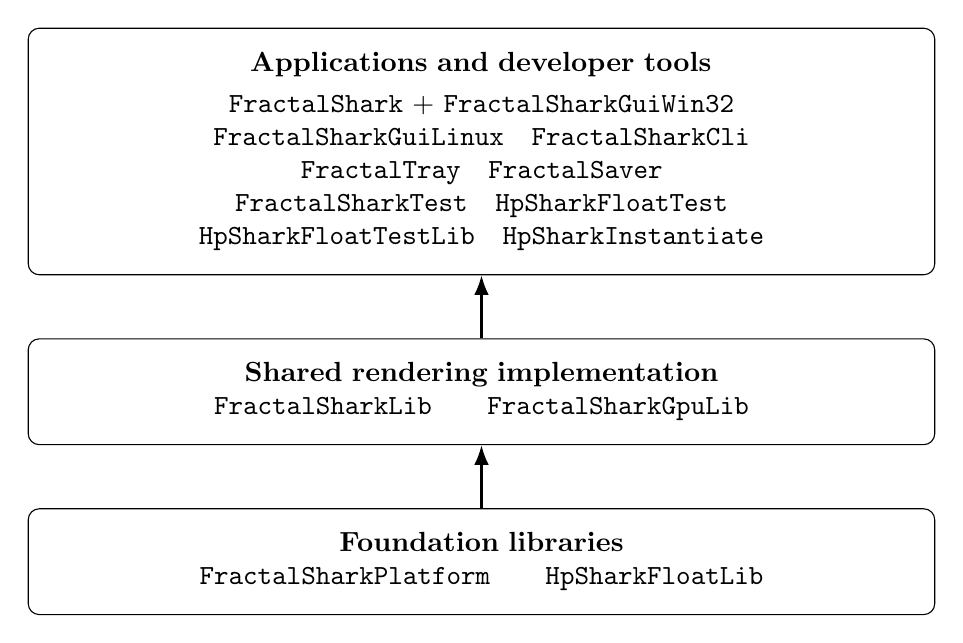
\begin{tikzpicture}[
      component/.style={
        draw,
        rounded corners,
        align=center,
        minimum height=12mm,
        text width=0.90\textwidth,
        inner sep=3mm
      },
      flow/.style={-{Latex[length=2.5mm]}, thick}
    ]
    \node[component] (foundation) {
      \textbf{Foundation libraries}\\
      \code{FractalSharkPlatform}\qquad \code{HpSharkFloatLib}
    };
    \node[component, above=8mm of foundation] (rendering) {
      \textbf{Shared rendering implementation}\\
      \code{FractalSharkLib}\qquad \code{FractalSharkGpuLib}
    };
    \node[component, above=8mm of rendering] (consumers) {
      \textbf{Applications and developer tools}\\[1mm]
      \code{FractalShark} + \code{FractalSharkGuiWin32}\quad
      \code{FractalSharkGuiLinux}\quad \code{FractalSharkCli}\\
      \code{FractalTray}\quad \code{FractalSaver}\quad
      \code{FractalSharkTest}\quad \code{HpSharkFloatTest}\\
      \code{HpSharkFloatTestLib}\quad \code{HpSharkInstantiate}
    };

    \draw[flow] (foundation) -- (rendering);
    \draw[flow] (rendering) -- (consumers);
  \end{tikzpicture}
  \caption[Codebase dependency layers]{Codebase dependency layers.  Platform and
    high-precision arithmetic support the shared CPU and CUDA rendering code;
    applications and validation tools consume those shared layers.}
  \label{fig:codebase-layers}
\end{figure}

\subsubsection{Foundation and rendering libraries}

\paragraph{\code{FractalSharkPlatform}.}
The platform library owns operating-system services used by otherwise portable
code.  Its common interfaces cover allocation, files, process information,
timing, diagnostics, crash handling, wait-cursor state, process memory limits,
and native OpenGL contexts.  Separate Win32 and Linux translation units provide
the implementations described in \cref{subsec:platform-abstraction}.

\paragraph{\code{HpSharkFloatLib}.}
The high-precision GPU arithmetic library implements the limb-based
\code{HpSharkFloat} representation, addition, NTT multiplication,
normalization, periodicity support, and the GPU reference-orbit machinery.  It
also contains the parameter families used to specialize those kernels.  The
numeric representation and execution pipeline are documented in
\cref{subsec:ref-orbit-gpu,subsec:hpfloat-model,sec:hp-add,sec:ntt-multiply}.

\paragraph{\code{FractalSharkLib}.}
The core library owns portable fractal state and CPU-side orchestration.  Its
responsibilities include coordinate conversion, reference-orbit dispatch,
linear-approximation construction, feature finding, palettes, iteration-buffer
management, render-thread coordination, persistence, PNG output, shared
commands, and functional tests.  The principal flows appear in
\cref{sec:ref-orbit-calc,sec:render-thread-pool,sec:disk_backed_growable_vectors}.

\paragraph{\code{FractalSharkGpuLib}.}
The rendering CUDA library owns the per-pixel launch surface and kernels for
direct escape-time rendering, perturbation, BLA and LA~v2 traversal,
antialiasing, coloring, and reductions.  It consumes numeric and state types
defined by the core and high-precision libraries; final applications link all
required libraries together.  Kernel behavior is covered in
\cref{sec:mandel-base-kernels,sec:perturb-only,sec:la-v2-perturb,sec:kernel-list}.

\subsubsection{Applications and front ends}

\paragraph{\code{FractalShark} and \code{FractalSharkGuiWin32}.}
The primary Windows application is split across two Visual~Studio projects.
\code{FractalShark} supplies the executable target, resources, icons, and final
link, while \code{FractalSharkGuiWin32} implements the Win32 entry point, main
window, command dispatcher, popup menus, console, saved-location UI, and splash
window.  Shared command identifiers remain in the core library.  User-visible
behavior and frame presentation are described in
\cref{sec:ui-popup-menu,sec:keyboard-shortcuts,subsec:opengl-display}.

\paragraph{\code{FractalSharkGuiLinux}.}
The native Linux application combines an Xlib event loop and menus, GLX context
management, Dear~ImGui overlays, clipboard integration, and the shared renderer.
Its platform boundary and current parity limitations are documented in
\cref{subsec:linux-gui}.

\paragraph{\code{FractalSharkCli}.}
The portable command-line executable provides headless rendering from built-in
views, saved locations, or explicit coordinates.  It exercises the same core
and CUDA rendering libraries without a window system; its contract and render
path are documented in \cref{sec:fractalshark-cli}.

\paragraph{\code{FractalTray}.}
The Windows tray application batch-renders a sequence of coordinates through
the shared renderer.  Its input format, configuration, and operating procedure
are described in \cref{subsec:fractaltray}.

\paragraph{\code{FractalSaver}.}
The Windows screen-saver project is legacy, unsupported code retained in the
Visual~Studio solution.  It is not part of the CMake build or release packages
and should not be treated as an active front end.

\subsubsection{Validation and generation tools}

\paragraph{\code{FractalSharkTest}.}
The portable unit-test executable covers core numeric types, coordinate
conversion, linear-approximation data, allocators, serialization, command
state, render goldens, and related utilities.  The custom test framework and
representative coverage are summarized in \cref{subsec:fractalsharktest}.

\paragraph{\code{HpSharkFloatTestLib} and \code{HpSharkFloatTest}.}
The support library contains reference implementations, correctness tests,
performance drivers, and result tracking for high-precision CUDA arithmetic.
The executable supplies the CUDA-aware harness that invokes those tests.
Runtime validation requires physical CUDA hardware, as discussed in
\cref{subsec:hpsharkfloattest}.

\paragraph{\code{HpSharkInstantiate}.}
The standalone developer tool generates explicit-instantiation CUDA sources
for the fixed \code{SharkFloatParams} families.  Generated translation units
control template compile time and final binary coverage; the underlying
strategy is documented in \cref{subsec:template-explicit-inst}.

\subsubsection{Build-system coverage}

The Visual~Studio solution contains the Windows application, Windows GUI
library, tray application, legacy screen saver, shared libraries, tests, and
generation tool.  CMake builds the portable shared libraries and tools,
\code{FractalSharkCli}, and \code{FractalSharkGuiLinux}; it intentionally omits
the Win32-only front ends.  Parallel project-file maintenance, Linux target
composition, and continuous-integration coverage are described in
\cref{subsec:dual-build}.

\input{FractalShark-B2-TemplateDesign}
\input{FractalShark-B3-TestsAndKernels}
\input{FractalShark-B4-DisplayPipeline}
\input{FractalShark-B5-ImaginaFormat}
\input{FractalShark-B6-CrossPlatform}

\section{Development History}
\label{sec:development-history}

This appendix records development notes that were posted over time.

\subsection{Release Notes}

\subsubsection{2026-9 News --- Version 0.543 (Upcoming)}

Version \code{0.543} improves repeated headless rendering and continues work on
the fused GPU reference-orbit implementation.

\begin{itemize}
\item \textbf{Persistent CLI server.} \code{FractalSharkCli} can now run as a
  server and accept repeated render requests from additional invocations of the
  same executable. The server retains initialized renderer state and processes
  requests in FIFO order. Local IPC uses named pipes on Windows and Unix-domain
  sockets on Linux.

\item \textbf{Asynchronous PNG output and timing.} Server renders begin PNG
  encoding in the background so encoding can overlap the next frame. Client
  output reports per-frame request time, while orderly server shutdown drains
  all outstanding encoders. A PowerShell example renders four deep-zoom scenes
  and reports total end-to-end time.

\item \textbf{GPU reference-orbit work.} The fused Ref2/v2 implementation
  receives further NTT, carry-propagation, memory-layout, and test-harness
  refinements.

\item \textbf{Build targets and platform support.} Release builds explicitly
  target compute capabilities 7.5, 8.0, 8.6, 8.9, 9.0, 10.0, and 12.0. Local
  builds default to compute capability 12.0 unless overridden. Windows and
  Linux remain fully supported at feature parity.
\end{itemize}

\subsubsection{2026-9-12 News --- Version 0.542}

\begin{itemize}
\item \textbf{CLI high-precision initialization.} The command-line renderer now
  initializes MPIR's default precision before parsing and converting locations,
  matching graphical-application initialization. This fixes flat direct-coordinate
  renders and precision failures at valid deep-zoom locations.
\end{itemize}

\subsubsection{2026-9-11 News --- Version 0.541}

\begin{itemize}
\item \textbf{CUDA architecture compatibility.} CUDA code generation now
  includes a compute-capability 7.5 target, restoring the fallback path used by
  RTX 3xxx cards and other supported GPUs without a matching native image.
\end{itemize}

\subsubsection{2026-9-7 News --- Version 0.54}

Version \code{0.54} replaces the original multi-kernel GPU high-precision
arithmetic path with the fused Ref2/v2 reference-orbit implementation.

\begin{itemize}
\item \textbf{Fused GPU reference orbit.} High-precision recurrence, NTT
  multiplication, signed carry propagation, normalization, and output run in a
  persistent cooperative CUDA kernel. The superseded standalone GPU add and
  multiply implementation is removed.

\item \textbf{GPU Newton--Raphson.} Feature-finder refinement uses the same
  fused high-precision machinery, including derivative accumulation and
  checkpoint validation against the CPU reference implementation.

\item \textbf{Extreme built-in views.} Views~\#33 and~\#34 exercise the new
  implementation at extreme depth. View~\#33's coordinates are corrected, and
  View~\#34 documents a feature at approximately $10^{650452}$ magnification.

\item \textbf{Validation and tooling.} GPU arithmetic tests, profiling tools,
  checksum diagnostics, and the technical notes are expanded around Ref2/v2.
\end{itemize}

\subsubsection{2026-7-4 News --- Version 0.532}

\begin{itemize}
\item \textbf{Rendering pipeline.} The render-thread pool and frame-publication
  path are refined, and parallel PNG saving is improved so output encoding can
  proceed without unnecessarily blocking subsequent rendering.

\item \textbf{Numeric performance.} HDR scaling operations receive a bitwise
  implementation that substantially reduces per-pixel overhead.

\item \textbf{Interaction fixes.} Feature autozoom is simplified around the
  stateless zoom-to-feature workflow. Palette rotation, context rendering,
  checkpoint metadata, OpenGL presentation, and startup behavior receive
  correctness fixes.

\item \textbf{Documentation.} The technical notes are reorganized into their
  current numbered sections and appendices.
\end{itemize}

\subsubsection{2026-6-27 News --- Version 0.531}

\begin{itemize}
\item \textbf{Shared graphical behavior.} Portable command handling, file
  operations, help content, saved locations, and menu-state logic are shared by
  the Win32 and Linux front ends. The Linux application is substantially
  simplified around the same contracts and reaches feature parity with Win32.

\item \textbf{Correctness fixes.} This release fixes a GPU normalization
  regression introduced between versions~0.51 and~0.52, a heap allocator false
  overrun report, repaint-state handling, and several GUI and numeric edge cases.

\item \textbf{Release packaging.} Continuous-integration artifacts and release
  packages are expanded, and project naming is made consistent across the two
  platforms.
\end{itemize}

\subsubsection{2026-6 News --- Version 0.53}

Version \code{0.53} introduced native Linux support.

\begin{itemize}
\item \textbf{Native Linux build.} The CMake + Clang build now covers the core
  numeric library, CUDA rendering, GPU high-precision arithmetic, tests, the
  command-line renderer, and the native graphical application. Debug and
  Release configurations are built in parallel with the Visual~Studio
  solution, and Linux release binaries are targeted at Ubuntu.

\item \textbf{Native Linux GUI.} \code{FractalSharkGuiLinux} now uses Xlib and
  GLX for its window and OpenGL presentation, a native hierarchical X11 popup
  menu, and Dear~ImGui overlays for help and application dialogs. Navigation,
  drag and wheel zoom, automatic zoom, feature finding, fullscreen transitions,
  clipboard output, and the principal save/load workflows are connected to the
  shared renderer and command catalog. The Linux and Win32 applications are
  fully supported and maintained at feature parity. Menu enablement, check
  marks, and radio selections are evaluated by the same portable implementation
  on both platforms.

\item \textbf{Portable platform services.} Operating-system dependencies are
  consolidated in \code{FractalSharkPlatform}, including allocation, files,
  process and memory queries, threading, input, diagnostics, wait cursors,
  embedded resources, and native OpenGL contexts. Shared library interfaces use
  portable window and geometry types instead of exposing Win32 types.

\item \textbf{Linux validation and packaging.} Linux CI builds Debug and
  Release, runs the portable CPU unit tests, smoke-tests the headless renderer,
  checks the release executables for unresolved dependencies, and packages
  \code{FractalSharkCli} with \code{FractalSharkGuiLinux}. CUDA-specific tests
  are compiled but remain a hardware validation step because hosted runners do
  not provide a physical GPU.
\end{itemize}

\subsubsection{2026-5-3 News --- Version 0.52}

Version \code{0.52} focuses on GPU-accelerated Newton--Raphson and begins the
cross-platform port to Linux.

\begin{itemize}
\item \textbf{GPU Newton--Raphson.}  A full GPU implementation of Newton's method
  for the feature finder is now integrated end-to-end: reference-orbit
  computation via NTT, first- and second-derivative accumulation, and
  convergence testing all run on the GPU.  An occupancy calculation bug is
  fixed, and a CPU-side ``reference reference orbit'' validates correctness
  against MPIR ground truth.

\item \textbf{Newton--Raphson checkpointing.}  The NR inner loop now supports
  save/resume with full-precision derivative state.  CPU and GPU checkpoint
  formats are compatible, so an interrupted computation can be resumed on
  either backend.

\item \textbf{Linux port (in progress).} A CMake + Clang build system is
  introduced alongside the existing Visual~Studio solution. At the time of
  this release, a GTK-based GUI was proposed and the port was incomplete.
  Version~0.53 superseded that proposal with the native Xlib/GLX and
  Dear~ImGui application described above. CPU-only unit tests already passed on
  Linux at this stage.

\item \textbf{Miscellaneous.}  Extracted \code{FeatureFinderOrchestrator} from
  the main class; improved the heap allocator panic path; parallelized the
  CI build; fixed Imagina file loading and RDP rendering regressions.
\end{itemize}

\subsubsection{2026-2-14 News --- Version 0.51}

Version \code{0.51} introduces the \textbf{Feature Finder} (\cref{sec:feature-finder}), a major new tool
for exploring the Mandelbrot set, along with several usability improvements.

\begin{itemize}
\item \textbf{Feature Finder.}  Move mouse near a feature, select feature
  finder, and \FractalShark{} will locate the nearest interesting feature---a
  mini-Mandelbrot or satellite bulb---using Newton's method (\cref{subsec:ff-newton}).  A line is drawn
  from the cursor to the detected feature, making its location visible.
  The finder works at any zoom depth.  Currently, the user manually chooses between
  direct iteration, perturbation theory, and linear approximation depending on
  the current zoom depth.  In the future, this choice will be automatic.

\item \textbf{Scan mode.}  Instead of a single click, scan mode surveys a grid
  of points across the screen and marks up to 144 discovered features with small
  circles.  This provides a quick overview of what is nearby before deciding
  where to zoom next.

\item \textbf{Auto-zoom to feature.}  Once a feature has been found the user can direct
  the program to zoom into it automatically.  The iteration count is ramped up
  smoothly during the zoom so the image stays sharp as the view approaches the target.
  This feature remains hacky and experimental but if it works it's fun to
  play with.

\item \textbf{Mouse-wheel zoom.}  Scroll the mouse wheel forward to zoom in
  toward the cursor, or backward to zoom out.  The code is rewritten.

\item \textbf{Rendering improvements.}  Parts of the OpenGL display layer are
  rewritten for better reliability and to support the new feature-finder
  overlays (lines and circles drawn on top of the fractal).

\item \textbf{Under the hood.}  Extended the derivative math in the
  linear-approximation pipeline so the feature finder works at extreme depths.
  Improved precision tracking during zoom.  Added a \code{.clang-format}
  configuration for consistent code formatting.
\end{itemize}

\subsubsection{2026-1-18 News --- Version 0.501}

\begin{itemize}
\item \textbf{Basic Wine compatibility.}  Tested without a GPU and working under
Wine 9.0 on Linux.   There are still some quirks, but basic rendering works in
CPU-only mode. Whether \FractalShark{} can work with Wine + CUDA remains unknown as
an appropriate test platform is not currently available.
\item \textbf{Proper fallback when no GPU is present.}  The program now detects lack of a CUDA
device and falls back to CPU-only rendering, with a warning message.
\item \textbf{Fixed some windowing bugs.}
\item \textbf{Improved these notes.}
\item \textbf{Linked at FractalForums.}  See \url{https://fractalforums.org/index.php?topic=5564.0}
\end{itemize}

\subsubsection{2025-12-29 News --- Version 0.5}
\begin{itemize}
  \item \textbf{GPU reference-orbit prototype.} Version~0.5 introduced the v1
  CUDA reference-orbit implementation, which used separate high-precision
  arithmetic phases.  That implementation has since been removed and
  superseded by the fused Ref2/v2 implementation documented in
  \cref{subsec:ref-orbit-gpu}.

  \item \textbf{Project plumbing.} Hooks up GitHub Actions to produce “official”
  builds, plus some refactoring; notes a startup windowing quirk.
\end{itemize}

\subsubsection{2025-07-28 News --- Version 0.46}

Version \code{0.46} was published as a pre-release, focusing on refactoring,
reference compression experimentation, save-file compatibility, and test infrastructure.

\begin{itemize}

  \item Continued internal \textbf{refactoring} of core rendering and control logic.
  
  \item Experimental support for \textbf{Imagina-style “max” reference compression},
        as an alternative to the existing “simple” scheme.
  
  \item Added preliminary support for \textbf{Imagina-compatible save files}.

  \item Enhanced internal \textbf{test infrastructure} with broader coverage and tooling.
    
  \item Work in progress toward additional infrastructure improvements.

\end{itemize}

This release was published on GitHub on July 28, 2025 (UTC) and is tagged as a
pre-release build.  


\subsubsection{2024-04-20 --- Version 0.45}

\begin{itemize}
  
  \item Adds a first cut at reference compression for an intermediate “perturbed
  perturbation” reference-orbit strategy.

  \item Includes three internal variants (v1: uncompressed/3 threads; v2:
  uncompressed/4 threads; v3: compressed/4 threads).

  \item v3 becomes the default at very deep “auto” perturbation settings;
  guidance given for when to stick to the older MT2 + periodicity workflow.

\end{itemize}


\subsubsection{2024-03-31 News --- Version 0.44}

Version \code{0.44} represents a substantial internal refactor emphasizing memory management, allocator control, and reference-orbit performance.

\begin{itemize}

  \item Removed the Boost dependency and introduced a custom
  \textbf{HighPrecision} wrapper.

  \item Improved reference-orbit performance, especially for low-precision,
  high-period locations.

  \item Improved performance of the \textbf{perturbed perturbation} algorithm.

  \item Introduced a custom file-backed \textbf{bump allocator} (\cref{sec:disk_backed_growable_vectors}) with stable
  interior pointers.

  \item Extended \code{GrowableVector} to support allocator-style usage
  without increasing committed memory.
  
  \item Updated reference orbit and linear approximation save-file formats.

  \item Added an \textbf{automatic perturbation mode} switching between single-threaded and multithreaded execution.

  \item Instrumented for memory-leak detection and fixed all known leaks.

  \item Fixed a long-standing correctness bug in BLAv1 dating back to version
  0.21.

  \item \textbf{Clarified ``perturbed perturbation'' design.} The implementation
  is framed as storing an intermediate-resolution reference orbit (e.g.\
  $\sim$500 bits), then using low-precision perturbation off that intermediate
  orbit to generate subsequent nearby reference orbits more efficiently.

\end{itemize}


\subsubsection{2024-03-03 News --- Version 0.43}
\begin{itemize}
  
  \item Significant performance wins for lower-precision, high-period
  reference-orbit computation.
  
  \item Adds a custom per-thread bump allocator for MPIR high-precision numbers.
  
  \item Rebalances work across the existing 3-thread multithreaded
  reference-orbit approach.

  \item \textbf{Allocator usage guidance.} The bump allocator is primarily
  beneficial for low-precision, high-period reference orbits; at very high
  precision the arithmetic dominates and allocation overhead is negligible. A
  suggested heuristic is to use the fixed-block bump allocator below roughly
  1000 digits and fall back to the global allocator above that.

  \item \textbf{Empirical sizing recommendation.} Tested successfully on a $\sim
  1\mathrm{e}{6000}$ location with about 4\,MB of bump-allocator space;
  recommendation is to use the smallest practical buffer (cache behavior matters).

  \item \textbf{Implementation refinement note.} In the current multithreaded
  orbit implementation, most allocations may occur on the main thread;
  thread-local allocation may be unnecessary. A few small allocator issues were
  identified for cleanup in the following release.

\end{itemize}


\subsubsection{2024-02-24 News --- Version 0.42}

Version \code{0.42} introduced major improvements to linear approximation performance, benchmarking, and configurability.

\begin{itemize}
  \item Added \textbf{multithreaded linear approximation table generation}.
  \item Significantly improved performance for high-period locations, especially with reference compression enabled.
  \item Added fine-grained benchmarking and performance breakdowns.
  \item Enabled regeneration of linear approximation tables independently of per-pixel data.
  \item Introduced adjustable linear approximation presets trading memory, accuracy, and performance.
\end{itemize}

This release corrected a prior precision regression and restored high-accuracy defaults.


\subsubsection{2024-01-15 News --- Version 0.41}

\begin{itemize}
  \item Fixes a minor bug in reference compression / GPU.
  \item Memory-use overhaul for storing LA tables and reference orbit to minimize RAM needed for hard views (e.g., View \#27).
  \item Default mode now uses temporary files + memory-mapped IO; avoids needing 2$\times$ memory during resize/copy and reduces committed-memory requirements with no measurable overhead per the release note.
\end{itemize}


\subsubsection{2024-01-01 News --- Version 0.4}

\begin{itemize}
  \item First working implementation of \textbf{runtime} reference compression
  (decompress-on-demand during rendering).

  \item Motivated as reducing end-to-end RAM requirements substantially on very
  high-period locations; not enabled by default for “Auto” rendering and
  described as work-in-progress.

  \item \textbf{Motivation: memory pressure.} Reference compression is
  explicitly framed as a response to high RAM requirements at difficult views
  (notably after enabling 64-bit iteration counts).
\end{itemize}


\subsubsection{2023-12 News --- Version 0.32}

Version \code{0.32} focused on usability, correctness, and incremental architectural cleanup.

\begin{itemize}
  \item Added \textbf{progressive rendering}, allowing partial image updates
  during long GPU renders.
  \item Added a \textbf{2x32 non-HDR linear approximation} path for numerically
  difficult shallow zooms.
  \item Fixed a subtle but severe correctness bug in the 2x32 implementation
  present in version 0.31.
  \item Added a basic regression test suite.
  \item Refactored code and restored buildability across inactive code paths.
\end{itemize}


\subsubsection{2023-12-09 News --- Version 0.31}

Version \code{0.31} expanded the set of available rendering algorithms and
substantially improved default performance at shallow and mid-depth zooms.

\begin{itemize}
  \item Added \textbf{1x32 linear approximation / perturbation} for
  high-performance shallow zooms.
  
  \item Added \textbf{1x64 linear approximation / perturbation}, primarily for
  correctness testing.
  
  \item Implemented \textbf{automatic render-algorithm selection} based on zoom
  depth.
  
  \item Eliminated unnecessary reference-orbit copying, significantly improving
  frame-to-frame performance.
  
  \item Fixed several bugs, including 2x32 correctness issues and unaligned
  HDRx64 memory access.

  \item \textbf{Auto-selection policy detail.} Auto mode is described as staging
  from direct 32-bit rendering at very shallow zooms, to 1x32 perturb-only, to
  1x32 LA, and finally 1x32 float-exp LA at deeper zooms, with the goal of
  improving default performance below roughly $10^{38}$.

  \item \textbf{Reference-orbit reuse optimization.} Removing unnecessary
  reference-orbit copying is called out as a major win for deep-zoom
  frame-to-frame responsiveness when reusing a reference orbit.

\end{itemize}


\subsubsection{2023-11-26 News --- Version 0.3}

\begin{itemize}
  
  \item Adds HDRx2x32 linear approximation: faster than LA/HDRx64 on consumer
  cards while retaining nearly native-64-bit precision.
  
  \item Notes that a “Debug View 20” anomaly is resolved under HDRx2x32,
  supporting the hypothesis that HDRx32 precision limits caused the issue.
  
  \item Misc performance improvements and bug fixes elsewhere.

  \item \textbf{Debug View 20 consistency improvement.} The ``Debug View 20''
  anomaly is reported as resolved under HDRx2x32, supporting the conclusion that
  the earlier HDRx32 behavior was a precision-limit issue.

  \item \textbf{HDRx2x32 precision characterization.} Described as ``Linear
  Approximation + Float EXP'' using a pair of 32-bit floats plus an exponent,
  with an estimated combined precision of roughly 46 bits.

\end{itemize}


\subsubsection{2023-11-12 News --- Version 0.24}

\begin{itemize}
\item \textbf{UI/UX improvements.} Adds a hotkey help view and general UI
cleanup.
\item \textbf{Random palette generation.} Adds a random palette generator; notes
the palette system remains intentionally constrained and may be expanded.
\item \textbf{Rendering diagnostics.} Adds a ``Show Rendering Details'' view for
inspecting current algorithm/settings.
\item \textbf{Early HDRx2x32 work.} Begins a GPU HDR 2x32 float implementation
(explicitly noted as not working yet).
\item \textbf{Crash diagnostics.} Automatically generates a crash dump on
unhandled exceptions.
\end{itemize}


\subsubsection{2023-11-05 News --- Version 0.23}
\begin{itemize}
  \item Adds switchable 64-bit iteration count support (enabling tens of
  billions of iterations per pixel, leveraging LA).
  \item Moves antialiasing/coloring into its own CUDA kernel for better
  performance.
  \item Multiple memory-reduction optimizations (systems-level) and related perf
  work.
  \item Adds reference-orbit save/load (no compression yet), useful for
  debugging deep spots.
  \item Notes a known bug manifesting in built-in View \#20 under a particular
  configuration (64-bit iterations + default HDRx32 LA~v2), with long render
  times due to slow reference-orbit calculation.
\end{itemize}


\subsubsection{2023-10-14 News --- Version 0.22}

\begin{itemize}

  \item Significant LA~v2 performance improvements (bug fixes); notes BLAv1 still
  winning in some cases.

  \item Fixes an LA~v2 correctness bug; release note claims no known correctness
  bugs remaining.

  \item \textbf{Performance data point.} Reports a minibrot example improving
  from roughly 470\,ms to 370\,ms (render-only; reference orbit excluded) on the
  author’s machine.

\end{itemize}


\subsubsection{2023-10-08 News --- Version 0.21}
\begin{itemize}
  \item Performance improvements to BLA and LA~v2.
  \item Memory-usage improvements (commit size / virtual address space issues
  called out).
  \item Generates more CUDA kernels for older GPUs (system requirements
  unchanged).
  \item Notes LA~v2 is strong for many deep-zoom cases but still behind older BLA
  in some shallower cases.
\end{itemize}


\subsubsection{2023-09-16 News --- Version 0.2}

Version \code{0.2} introduced a major algorithmic milestone: the integration
of Imagina's linear approximation implementation as a CUDA kernel.

\begin{itemize}
  \item Added Imagina-based linear approximation (\code{LAv2}), now the
  default rendering algorithm.
  \item Resolved known correctness bugs in the new approximation path.
  \item Fixed a major performance regression caused by an earlier implementation oversight.
  \item Achieved large performance gains at deeper zoom levels compared to the
  existing bilinear approximation.
\end{itemize}

While the legacy bilinear approximation remains faster at very shallow zooms,
the new approach dominates once meaningful magnification is reached.


\subsubsection{2023-07-22 News --- Version 0.11}

Version \code{0.11} was released with a focus on performance improvements and
improved diagnostics.

\begin{itemize}
  \item Approximately \textbf{+10\% performance improvement} in the HDRx32 CUDA
  rendering path.
  \item Fixed several minor bugs affecting correctness and stability.
  \item Improved CUDA error reporting by displaying descriptive error strings
  instead of numeric codes.
\end{itemize}

A long-duration technology demonstration video accompanied this release,
showcasing a zoom to approximately $10^{4000}$ using the default HDRx32/BLA CUDA
kernel.  Rendering and post-processing each required roughly one and a half
days.


\phantomsection
\addcontentsline{toc}{section}{References}
\bibliographystyle{plain} % or ieeetr, unsrt, alpha, etc.
\bibliography{FractalShark}      % <-- filename WITHOUT .bib

\end{document}
